\chapter{1. Contexto, práticas e elementos de linguagem}

\colorsec{Habilidades do SAEB}

\begin{itemize}
  \item Reconhecer artistas que contribuíram para o desenvolvimento e a disseminação de diferentes gêneros e estilos nas artes visuais, dança, música e teatro.
  \item Analisar formas, gêneros e estilos distintos de artes visuais e dança, em diferentes contextos, por meio de seus elementos constitutivos.
  \item Analisar a função do tema como projeto integrador das diferentes linguagens artísticas.
\end{itemize}

\colorsec{Habilidades da BNCC}

\begin{itemize}
  \item EF69AR01, EF69AR03, EF69AR04.
\end{itemize}


\conteudo{Para entendermos o que significa ``contexto da obra de arte'', primeiramente é preciso entender o que significa o verbo ``contextualizar'': mostrar as circunstâncias que estão ao redor de um fato, um acontecimento ou uma situação; entender ou interpretar
algo tendo em conta as circunstâncias que o rodeiam.

Tendo como base esse significado, podemos entender que, para
contextualizar, é necessário analisar, interpretar e compreender uma obra
de arte, sabendo que ela foi elaborada pelos sujeitos a partir de
determinados momentos sociais, culturais e históricos em que vivem ou
viveram. A linguagem artística utilizada pelos sujeitos revela-se uma
entre outras práticas sociais e, portanto, guarda relação com a
história, com a cultura e com a sociedade de cada grupo.

Como atividade dinâmica e socialmente produzida, a linguagem artística
está sujeita a mudanças, reformulações e variantes que dizem respeito à
identidade dos sujeitos que a produzem, assim como às condições do
ambiente, aos objetivos, às funções e à época em que está sendo
empregada.

Para ajudar na contextualização de uma obra de arte, devem-se fazer perguntas como: em que data a obra foi realizada? A que período histórico a
obra está relacionada? Que artista a realizou? O que sabemos ou podemos
saber sobre esse artista? Com que finalidade a obra foi realizada? Que
os fatos sociais, políticos, econômicos, religiosos e culturais são mais
marcantes no período em que a obra foi produzida? Que relações a obra
poderia estabelecer com esses fatos? A que movimento artístico a obra
está relacionada? Quais características desse movimento estão presentes
na obra ou quais não estão?

Já as práticas na arte são o fazer artístico. Trata-se do colocar mãos à obra e experimentar e vivenciar
a arte como uma prática social, interagindo com a linguagem artística,
não somente como expectador (analista ou apreciador), mas como criador (sujeito ativo).

Por outro lado, sem intenção de esgotar os múltiplos elementos da linguagem
artística, podemos citar:

\textbf{Artes visuais}: ponto, linha, forma,
direção, cor, tom, escala, dimensão, espaço, movimento.

\textbf{Música}: altura, intensidade, timbre, melodia, ritmo. 

\textbf{Teatro}: entonações de voz, personagens, enredo, figurinos, cenário, iluminação,
sonoplastia.

\textbf{Dança}: tempo, peso, fluência, espaço, deslocamentos,
ritmos de movimento, direções.}


\colorsec{Atividades}

\num{1}  Para analisar e compreender uma obra de arte, o que se faz necessário?

\linhas{4}
\coment{É necessário saber que ela foi elaborada pelos sujeitos a partir de
determinados momentos sociais, culturais e históricos em que vivem ou
viveram.}

\num{2} Como deve ser a interação do sujeito com a linguagem artística?

\linhas{4}
\coment{O sujeito deve experimentar e vivenciar a arte como uma prática social,
interagindo com a linguagem artística, não somente como expectador --- ou seja,
analista ou apreciador ---, mas também como criador --- ou seja, sujeito ativo.}

\num{3}  Cite três elementos da linguagem artística que compõem cada item destacado a seguir.

\begin{escolha}
\item
  Artes visuais: \preencher, \preencher e \preencher.

\coment{ponto, linha, forma, direção, cor, tom, escala, dimensão, espaço,
movimento}

\item
  Dança: \preencher, \preencher e \preencher.

\coment{tempo, peso, fluência, espaço, deslocamentos, ritmos de movimento,
direções}

\item
  Música: \preencher, \preencher e \preencher.

\coment{altura, intensidade, timbre, melodia, ritmo}

\item
  Teatro: \preencher, \preencher e \preencher.

\coment{entonações de voz, personagens, narrativas, figurinos, cenário,
iluminação, sonoplastia}
\end{escolha}

\num{4} Analise os itens propostos a seguir.

\begin{itemize}
  \item Na Grécia Antiga, surgiram dois gêneros: a tragédia e a comédia.
  \item Na Grécia Antiga, a arte era apresentada em espaços especiais,
construções em forma de meia-lua.
  \item Na Itália, no final da Idade Média e início do Renascimento, surge a
\textit{commedia dell'arte}, com textos improvisados.
  \item O nome da manifestação artística deriva de um verbo grego que significa algo como ``ver'' ou ``enxergar'' e significa ``lugar de onde se vê''.
\end{itemize}

Os itens relacionam-se à que manifestação artística?

\linhas {2}
\coment{Trata-se do teatro.}

\num{5} Divida-se com seus colegas em quatro grupos e realize a atividade proposta a seguir.

\begin{escolha}
  \item Cada grupo deverá pesquisar e estudar um período específico da história do teatro: \textbf{teatro na Antiguidade} (origens e teatro grego); \textbf{teatro na Idade Média} (teatro litúrgico e teatro medieval); \textbf{Renascimento e teatro Elisabetano} (renascimento teatral na Europa e o teatro de William Shakespeare); \textbf{teatro moderno e contemporâneo} (teatro realista, teatro do absurdo e teatro contemporâneo).
  \item Cada grupo deve pesquisar sobre o período designado, levantando informações sobre as principais características, os autores, as obras e asinfluências teatrais da época.
  \item Os grupos devem preparar uma apresentação oral, na qual cada membro do grupo terá a oportunidade de compartilhar suas descobertas.
  \item Durante a apresentação de um grupo, os demais grupos devem fazer anotações sobre os aspectos mais interessantes e fazer perguntas para estimular a discussão.
\end{escolha}

Após todas as apresentações, promovam um debate em sala de aula, abordando os seguintes pontos:

\begin{itemize}
  \item Como o teatro reflete as características culturais e sociais de cada período estudado?
  \item Quais foram as principais transformações e os avanços ocorridos ao longo da história do teatro?
  \item Como o teatro se adaptou às mudanças tecnológicas e sociais ao longo dos séculos?
  \item Quais são as influências do teatro passado no teatro contemporâneo?
  \item Como o teatro contribui para a nossa compreensão da história e da sociedade?
\end{itemize}

Redija um pequeno texto comentando a atividade proposta como um todo.

\linhas{10}
\coment{Ao dividir a turma em grupos e atribuir a cada um um período específico da história do teatro, proporciona-se aos alunos a oportunidade de se aprofundarem em uma área específica e se tornarem especialistas temporários. Isso não só os incentiva a pesquisar e adquirir conhecimento, mas também os encoraja a compartilhar suas descobertas com os colegas. A dicussão em sala de aula, após as apresentações, é um elemento valioso para a compreensão mais ampla do teatro ao longo do tempo. As perguntas instigam os alunos a refletir criticamente sobre as influências históricas, as transformações teatrais e o impacto do teatro em diferentes sociedades. A atividade não só promove o aprendizado de conteúdo, mas também habilidades de pesquisa, apresentação oral, trabalho em equipe e pensamento crítico.}

\num{6} O corpo se expressa nas artes visuais, na dança, na música, no
teatro e é representado de muitas formas. Sobre o assunto, analise as descrições apresentadas a seguir. Depois, pesquise e registre uma manifestação artística visual que se relaciona a cada descrição proposta.

\begin{escolha}
\item Corpo feito com poucas linhas, pouca profundidade, para expressar
a religiosidade e esconder a sensualidade de corpos reais.

\linhas{4}
\coment{Possibilidade de resposta: \textit{Madonna Rucellai}, de Duccio di Buoninsegna, de 1285. Disponível em: https://commons.wikimedia.org/wiki/File:Madonna_em_Majestade_dita_Rucellai_-_Duccio.jpg. Acesso em: 10 maio 2023.}

\item Corpo representando figura de destaque na sociedade, uma forma de
cultuar os mortos, com linhas simples e níveis retilíneos.

\linhas{4}
\coment{Possibilidade de resposta: máscara funerária egípcia. Disponível em: https://commons.wikimedia.org/wiki/File:Funerary_Mask_of_Wah_MET_DP311797.jpg. Acesso em: 10 maio 2023.}

\item Corpo simplificado, feito com poucas linhas, que sugere a prática de
punições daquela cultura.

\linhas{4}
\coment{Possibilidade de respsota: pintura rupestre da Serra da Capivara. Disponível em: https://commons.wikimedia.org/wiki/File:Puni\%C3\%A7\%C3\%B5es_(14205232887).jpg. Acesso em: 10 maio 2023.}

\item Corpo humano representado dentro das proporções corretas, para
expressar os ideais da sociedade da época, de harmonia e de 
equilíbrio.

\linhas{4}
\coment{Possibilidade de resposta: \textit{Discóbolo}, de Míron, do século V a.C. Disponível em: https://commons.wikimedia.org/wiki/File:Roman_bronze_copy_of_Myron\%E2\%80\%99s_Discobolos,_2nd_century_CE_(Glyptothek_Munich).jpg. Acesso em: 10 maio 2023.}
\end{escolha}

\num{7} Sobre os elementos constitutivos das artes visuais, marque V para
verdadeiro e F para falso.

\begin{boxlist}
\item Os elementos que compõem as artes visuais são quatro: ponto, cor, linha e forma. \coment{F}

\item O ponto é um dos elementos da linguagem visual. Uma série de pontos forma uma linha; e uma massa de pontos torna-se textura, forma ou plano. \coment{V}

\item As linhas, sequências ordenadas de pontos, podem ser retas ou curvas. \coment{V}

\item No espaço bidimensional, as formas têm altura, largura e profundidade. \coment{F}
\end{boxlist}

\num{8} Associe o gênero de cada arte visual a uma característica.

\begin{itemize}
  \item I. Autorretrato.
  \item II. Paisagem.
  \item III. Natureza-morta.
  \item IV. Retrato.
\begin{itemize}

\begin{escolha}
  \item Representação de qualquer objeto inanimado. \coment{III}
  \item Representação de um local, seja no campo, seja na cidade. \coment{II}
  \item Representação de alguém por um artista. \coment{IV}
  \item Representação do artista por si mesmo. \coment{I}
\end{escolha}

\num{9} Leia o texto.

\begin{quote}
A linguagem audiovisual é uma combinação de elementos sonoros e visuais. Esses artefatos culturais impactam os sentidos da visão e da audição do ser humano.

\fonte{Texto escrito para este material.}
\end{quote}

Cite três elementos constitutivos das linguagens das artes visuais que
se integram à linguagem audiovisual do cinema.

\linhas{4}

\coment{Possibilidade de resposta: cor, espaço, movimento, luz, sombra, tom, som.}

\num{10} Leia o texto sobre Augusto Boal.

\begin{quote}
\textbf{Augusto Boal}

Augusto Boal, um dos grandes nomes da dramaturgia brasileira, deixou um legado duradouro mesmo após sua morte aos 78 anos de idade. Sua abordagem inovadora do teatro como uma ferramenta de luta política e social o destacou no cenário artístico. Boal é conhecido como o criador do Teatro do Oprimido, uma técnica que coloca os espectadores como protagonistas nas encenações, rompendo as barreiras entre realidade e ficção.

Além de suas contribuições teatrais, Boal também se destacou como autor de diversas obras literárias. Seu impacto transcendeu fronteiras, conquistando prêmios e honrarias tanto no Brasil quanto no mundo. Em 2009, ano de seu falecimento, ele foi nomeado Embaixador Mundial do Teatro pela UNESCO, reconhecimento merecido por seu compromisso com a arte e sua capacidade de promover mudanças sociais através do teatro.

\fonte{Fonte de pesquisa: Luciana Console. Brasil de Fato. Há 10 anos, falecia Augusto Boal, criador do Teatro do Oprimido. Disponível em:
\emph{https://www.brasildefato.com.br/2019/05/02/ha-10-anos-falecia-augusto-boal-criador-do-teatro-do-oprimido}.
Acesso em: 08 mar. 2023.}
\end{quote}

Assim como Augusto Boal, no Brasil vários artistas contribuíram para o
desenvolvimento e a disseminação de diferentes gêneros e estilos no
teatro, nas artes visuais, na dança e na música. Faça uma pesquisa sobre os artistas elencados a seguir para escrever brevemente sobre eles e suas contribuições.

\begin{escolha}[]{@{}ll@{}}
  \item Amilcar de Castro.

\linhas{10}
\coment{Amilcar de Castro (1920-2002) foi um renomado escultor brasileiro que deixou um legado marcante no mundo das artes. Sua obra é caracterizada por formas geométricas minimalistas, explorando a relação entre o vazio e o sólido, e convidando o espectador a interagir com suas esculturas. Utilizando principalmente o aço, suas peças revelam uma estética elegante e precisão técnica. Amilcar de Castro é reconhecido nacional e internacionalmente, tendo exposto em galerias e museus ao redor do mundo. Sua contribuição para a arte contemporânea brasileira é amplamente admirada e inspiradora, fazendo dele um dos artistas mais importantes do país.}

  \item Deborah Colker.

\linhas{10}
\coment{Deborah Colker é uma renomada coreógrafa e bailarina brasileira conhecida por suas criações inovadoras na dança contemporânea. Fundadora da Deborah Colker Companhia de Dança, ela combina movimento, música e cenografia de maneira única. Sua abordagem criativa inclui diferentes estilos e técnicas de dança, resultando em performances expressivas e técnicas. Colker colabora com artistas de diversas áreas e é reconhecida nacional e internacionalmente por sua contribuição à dança contemporânea.}

  \item Pixinguinha.

\linhas{10}
\coment{Pixinguinha foi um renomado músico brasileiro, conhecido por sua contribuição ao choro. Compositor, arranjador, flautista e saxofonista, ele revolucionou a música brasileira ao incorporar elementos do jazz e da música erudita. Suas composições, como "Carinhoso" e "Lamentos", são consideradas clássicos do repertório brasileiro. Pixinguinha liderou conjuntos importantes, como Os Oito Batutas, e seu legado continua influenciando músicos até hoje. Sua genialidade e contribuição o tornaram uma figura icônica da música brasileira.}


\colorsec{Treino}

\num{1} Leia o texto.

\begin{quote}
A instalação \textit{Canções esquecidas}, do artista australiano Michael Thomas Hill, consiste em diferentes gaiolas penduradas sobre uma área grande. Sob as gaiolas, podem-se ouvir os sons dos pássaros que habitaram Sydney, na Austrália, antes da urbanização da cidade.

\fonte{Texto escrito para este material.}
\end{quote}

Com base na descrição, percebe-se que a instalação do artista australiano

\begin{escolha}
\item
  permite o diálogo entre diferentes linguagens e a interação com o
  público.
\item
  tem como principal característica ser efêmera (só existir durante o
  tempo destinado àquela exposição).
\item
  relaciona-se à arte moderna e pode ser montada em museus, galerias e
  espaços abertos.
\item
  espera que o espectador participe passivamente da obra, comportando-se apenas como
  apreciador.
\end{escolha}

\coment{SAEB: Analisar formas, gêneros e estilos distintos de artes visuais e
dança, em diferentes contextos, por meio de seus elementos
constitutivos.
BNCC: EF69AR01 -- Pesquisar, apreciar e analisar formas distintas das artes visuais tradicionais e
contemporâneas, em obras de artistas brasileiros e estrangeiros de diferentes épocas e em
diferentes matrizes estéticas e culturais, de modo a ampliar a experiência com diferentes
contextos e práticas artístico-visuais e cultivar a percepção, o imaginário, a capacidade de
simbolizar e o repertório imagético.

a) Correta. Na instalação, há o diálogo entre diferentes linguagens e a
interação com o público, que percorre o espaço percebendo a obra de
vários ângulos e com os diferentes sentidos.
b) Incorreta. A instalação pode ter um caráter efêmero, só existindo no
período determinado para a exposição, ou pode ser desmontada e recriada
em outro local.
c) Incorreta. Não se relaciona com a arte moderna, pois é uma linguagem
artística que surgiu a partir dos anos 1960, ou seja, é arte
contemporânea.
d. Incorreta. O espectador participa ativamente da obra, e não se
comporta somente como apreciador.}

\num{2} Leia o texto.

\begin{quote}
\emph{O gabinete do dr. Caligari} aponta o esgotamento físico, emocional e moral dos alemães após a Primeira Guerra Mundial. O filme, de 1920, é marcado por
cenários irreais, com foco no interior, atuações e caracterizações
exageradas, imagens com ângulos profundos e sombras marcantes, usando a
iluminação e os ângulos da câmera para criar atmosferas de medo, horror,
dor.

\fonte{Texto escrito para este material.}
\end{quote}

Com base no texto, assinale a alternativa que corresponde ao movimento artístico a que esse filme se liga.

\begin{escolha}
\item
  Impressionismo.
\item
  Expressionismo.
\item
  Surrealismo.
\item
  Neorrealismo.
\end{escolha}

\coment{SAEB: Analisar a função do tema como projeto integrador das diferentes
linguagens artísticas.
BNCC: EF69AR03 -- Analisar situações nas quais as linguagens das artes visuais se integram às
linguagens audiovisuais (cinema, animações, vídeos etc.), gráficas (capas de livros, ilustrações
de textos diversos etc.), cenográficas, coreográficas, musicais etc.

a) Incorreta. Apesar de, no cinema, o Impressionismo ser do mesmo período temporal que o Expressionismo,
a estética é diferenciada. No impressionismo, o foco da filmagem é no
exterior, no ângulo subjetivo (olhar do personagem). Esse movimento teve
início na França.
b) Correta. O filme \emph{O gabinete do dr. Caligari} é do movimento
expressionista alemão e possui como características o foco da filmagem
no interior, a morbidez temática e a interpretação teatral.
c) Incorreta. O movimento surrealista do cinema também é do mesmo
período temporal (1920-1930) e teve início na França.
d. Incorreta. O neorrealismo italiano surgiu na década de 1940 e buscava
descrever de forma fiel a vida nos anos de guerra. As filmagens eram
feitas nas ruas.}

\num{3}  Leia o texto.

\begin{quote}
O abstracionismo, em termos gerais, engloba formas de arte que não seguem a figuração ou a imitação do mundo. Em um sentido mais específico, o termo está associado às vanguardas europeias das décadas de 1910 e 1920, que rejeitaram a representação ilusionista da natureza. Características comuns das diferentes correntes abstratas incluem a decomposição da figura, a simplificação da forma, o uso inovador da cor, a rejeição da perspectiva e das técnicas tradicionais de modelagem, assim como a recusa aos jogos convencionais de luz e sombra.

\fonte{Fonte de pesquisa: Editores da Enciclopédia Itaú Cultural. Enciclopédia Itaú Cultural. Abstracionismo. Disponível em:
\emph{https://enciclopedia.itaucultural.org.br/termo347/abstracionismo}.
Acesso em: 08 mar. 2023.}
\end{quote}

O nome de um expoente desse estilo é

\begin{escolha}
\item Leonardo da Vinci.

\item Frida Kahlo.

\item Piet Mondrian.

\item Vincent Van Gogh.
\end{escolha}

\coment{SAEB: Reconhecer artistas que contribuíram para o desenvolvimento e a
disseminação de diferentes gêneros e estilos nas artes visuais, dança,
música e teatro.
BNCC: EF69AR04 -- Analisar os elementos constitutivos das artes visuais (ponto, linha, forma, direção,
cor, tom, escala, dimensão, espaço, movimento etc.) na apreciação de diferentes produções
artísticas.

a) Incorreta. Leonardo da Vinci é representante da arte renascentista.
Suas obras são regidas pela figuração e pela imitação do mundo.
b) Incorreta. As obras de Frida Kahlo eram regidas pela figuração
estilizada.
c) Correta. Piet Mondrian (1872-1944), pintor holandês, é um dos maiores
representantes do abstracionismo geométrico.
d) Incorreta. Vincent Van Gogh utilizava em suas obras arte figurativa
estilizada.}

\chapter{2. Materialidades, notação e registros musicais}

\conteudo{\textbf{Materialidades}

A materialidade na obra de arte é constituída por elementos visuais, ou
seja, é formada, principalmente, por aquilo que podemos ver, e também
pelo que podemos apreender por meio dos sentidos; compor, conceber,
criar.

Como exemplos de materialidades, podemos citar nas artes plásticas: a
tela (suporte), o pincel (ferramenta) e a tinta (matéria); na música:
sujeito que toca ou canta (suporte), instrumentos musicais (ferramenta)
e os sons (matéria); na dança e no teatro: o corpo do artista (suporte e
ferramenta) e os gestos (matéria).

\textbf{Notação e registros musicais}

Segundo o dicionário Michaelis on-line, notação musical é a
``representação por meio de sinais, do tom e duração dos sons, e
marcação das suspensões e pausas''.

A notação musical é um sistema de símbolos, um sistema gráfico, que
permite a leitura de uma composição musical, podendo representar
elementos de uma composição musical como altura, duração, intensidade e
timbre.

São exemplos de notações musicais:

\begin{itemize}
\item
  Partitura - sistema de escrita musical tradicional e padronizado
  mundialmente, com cinco linhas e quatro espaços em branco, símbolos
  para as notas musicais, pausas, entre outros elementos.
\item
  Tablatura -- sistema de escrito musical que informa a tecla ou o lugar
  onde o dedo do intérprete deve ser posicionado para tocar a composição
  musical, utilizando para isso letras ou números.
\end{itemize}
}

\coment{
Neste módulo, os alunos retomam conteúdos, aprendizagens e experiências
sobre os objetos de conhecimento: contextos e práticas e elementos da
linguagem, ampliando suas análises e reflexões, tendo, também, como base
outros objetos de conhecimento do componente arte: materialidades e
notação e registro musical.

Sugerimos que a primeira leitura do texto seja realizada pelos alunos
individualmente. Depois, faça a leitura em voz alta do texto, fazendo
duas pausas, sugeridas a seguir.

Pausa 1 -- leitura do trecho sobre materialidades. Peça aos alunos que
expliquem o que entenderam por suporte, ferramenta e matéria. Caso
tenham dificuldade, auxilie-os a compreender o que está sendo denominado
como:

\begin{itemize}
\item
  suporte (o que sustenta, suporta, segura a obra de arte);
\item
  ferramenta (instrumento, recurso tecnológico utilizado para a
  criação);
\item
  matéria (é o material utilizado durante a criação).
\end{itemize}

Pausa 2 -- leitura do trecho sobre notação e registros musicais.
Sugerimos que você apresente, por meio de projeção ou impressão, ao
menos um exemplo de partitura e tablatura, para que os alunos possam
relembrar e analisar como são feitos os registros gráficos do som nesses
dois sistemas de escrita musical.\\
\textbf{Habilidades BNCC}: EF69AR09 / EF69AR10 / EF69AR16 / EF69AR18 /
EF69AR20 / EF69AR21 / EF69AR22 / EF69AR24
}

\colorsec{Habilidades SAEB}

\begin{itemize}
\item Identificar diferentes formas de registro das artes por meio de
notação ou procedimentos e técnicas de áudio e audiovisual.

\item Identificar os usos de diferentes tecnologias e recursos digitais na
produção e circulação das linguagens artísticas.

\item Analisar formas, gêneros e estilos distintos de música e teatro em
diferentes contextos, por meio de seus elementos constitutivos.

\item Analisar o papel dos profissionais e a utilização dos equipamentos
culturais no sistema de produção e circulação das artes visuais, dança,
música e teatro.
\end{itemize}

\colorsec{Atividades}

\num{1} Marque com C a alternativa que corresponde à notação musical
convencional e com NC à notação musical não convencional.

%( C ) 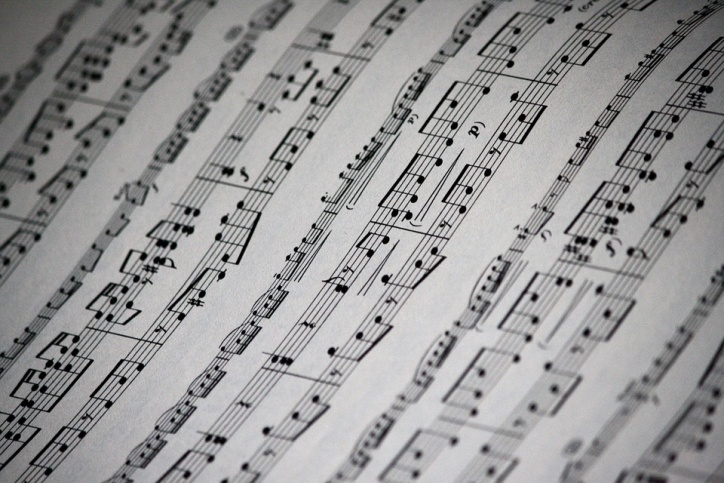
\includegraphics[width=3.29167in,height=2.19444in]{media/image11.jpeg}

%https://pixabay.com/pt/photos/partitura-notas-m\%c3\%basica-textura-1327003\textgreater{}\strut

%( NC )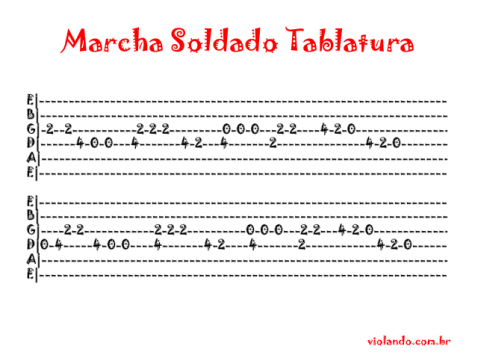
\includegraphics[width=4.71959in,height=2.08333in]{media/image12.png}
%Editora, refazer essa imagem de tablatura. A imagem de referência encontra-se disponível em: https://violando.com.br/tablatura.

%( NC ) 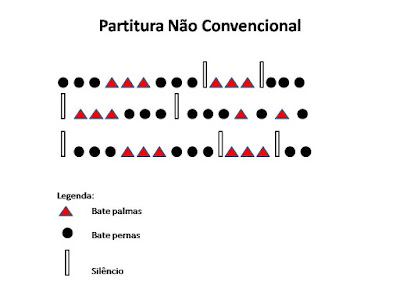
\includegraphics[width=4.16667in,height=2.57292in]{media/image13.jpeg}

%Editora, refazer imagem. Imagem de base encontra-se disponível em: http://adriartessempre.blogspot.com/2017/08/partitura-convencional-e-nao.html

%( C ) 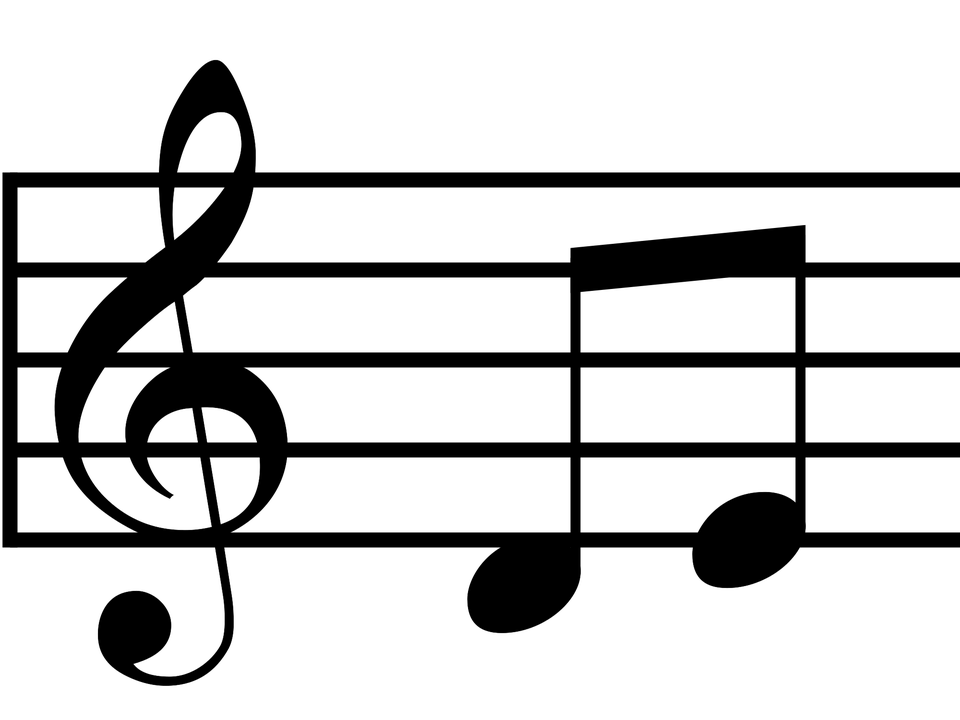
\includegraphics[width=1.50000in,height=2.44792in]{media/image14.png}

%https://pixabay.com/pt/illustrations/nota-musical-png-clave-de-sol-chave-1275607

\coment{
Saeb: - Identificar diferentes formas de registro das artes por meio de
notação ou procedimentos e técnicas de áudio e audiovisual.

Habilidade BNCC: EF69AR22

Ordem das respostas:

C: No sistema de notação musical tradicional o elemento básico da
partitura é a pauta (pentagrama). A pauta consiste em cinco linhas
paralelas e quatro espaços, onde é possível colocar diversas informações
da música: as notas musicais que compõem a melodia, o tom, a
intensidade, o ritmo, o andamento e as harmonias;
NC: Trata-se de uma notação musical não convencional, uma tablatura para
violão. Cada linha representa uma corda do instrumento. Os números
representam as casas onde devemos prender as notas. As letras
representam as linhas. Na ilustração, encontra-se representada a
tablatura da música ``Marcha soldado''. Para tocar essa música faz-se
necessárias apenas duas cordas: G (terceira corda -- sol) e D (quarta
corda -- ré);
NC: Essa notação contemporânea e criativa tem, geralmente, como objetivo
iniciar crianças na leitura de símbolos musicais diferentes daqueles da
notação musical tradicional;
T: Trata-se da clave de sol, um dos símbolos mais conhecidos da notação
musical tradicional.

Indicação de sites:

https://musopen.org/pt/sheetmusic/ - Possui mais de 100 mil
partituras disponíveis em PDF para vozes e vários instrumentos musicais,
com download gratuito.

HTTPS://imslp.org/ - A Biblioteca Musical
Petrucci contém um acervo de partituras e gravações de músicas em
domínio público, disponíveis para download.}

\num{2} Leia o texto.

\section{O pai do samba: o lundu}

\begin{quote}
O lundu (landum, lundum, londu) é dança e canto de origem africana
introduzido no Brasil provavelmente por escravizados de Angola. Da mesma
forma que a modinha, há inúmeras controvérsias quanto à sua origem.
Confundido inicialmente com o batuque africano (do qual proveio),
tachado de indecente e lascivo nos documentos oficiais, que proibiam sua
apresentação nas ruas e teatros. {[}...{]}

Como dança, a coreografia do lundu foi descrita como tendo certa
influência espanhola pelo alteamento dos braços e estalar dos dedos,
semelhante ao uso de castanholas, com a peculiaridade da umbigada, ponto
culminante do encontro lascivo dos umbigos do homem e da mulher na
dança. Traço característico e predominante em sua evolução seria o
acompanhamento marcado por palmas, num canto de estrofe-refrão típico da
cultura africana.~{[}...{]}

Como gênero de música cantada, a mais antiga menção ao lundu-canção é
encontrada nos versos de Caldas Barbosa que, além da modinha brasileira,
implantou na Corte portuguesa a moda do lundu cantado a viola.

\fonte{Disponível em:
https://institutocravoalbin.com.br/o-pai-do-samba-o-lundu. Acesso
em: 9 mar. 2023.}
\end{quote}

Sobre o texto que você leu podemos afirmar que

\begin{escolha}
\item
  o~lundu é um gênero musical erudito e uma dança brasileira de
  natureza híbrida.
\item
  o lundu aproveitou características de danças africanas, como o estalar
  dos dedos.
\item
  o dançarino, suporte e a ferramenta da dança lundu, executa gestos e
  movimentos que revelam significados do seu contexto
  histórico-sócio-cultural.
\item
  o samba é considerado o gênero que influenciou o lundu.
\end{escolha}

\coment{Saeb: - Analisar formas, gêneros e estilos distintos de música e teatro
em diferentes contextos, por meio de seus elementos constitutivos.

Habilidades BNCC: EF69AR16 / EF69AR18

a) Incorreta. O lundu é um gênero musical contemporâneo;
b) Incorreta. O lundu aproveitou características de danças europeias;
c) Correta. Em relação às materialidades, o dançarino, é o suporte e
ferramenta da dança. O texto deixa claro o momento histórico: período
colonial brasileiro e como a sociedade se organizava em relação à
cultura dos escravizados;
d) Incorreta. O lundu é considerado o pai do samba.}

Para responder às atividades 3 e 4, leia o texto.

%\textless{}Fazer uma montagem com as duas fotos indicadas a seguir.\textgreater{}

Isadora Duncan, bailarina e coreógrafa estadunidense, procurava
inspiração nos movimentos da natureza, como o fluir das ondas do mar.
Fotos do início do século XX.

%\textless{}\emph{\url{https://commons.wikimedia.org/wiki/File:Isadora_Duncan3.jpg}
%\textless{}\emph{\url{https://commons.wikimedia.org/wiki/File:Isadora_Duncan2.jpg}

\begin{quote}
O expressionismo, movimento estético do início do século XX, teve
expoentes em diversas áreas no mundo das artes: na dança, no cinema, na
literatura, na arquitetura, na escultura, na música.

Esse movimento surgiu como uma reação à representação objetiva do
impressionismo, no contexto histórico da Primeira Guerra Mundial e da
sociedade moderna, industrializada, buscando expressar sentimentos e
emoções, utilizando a arte para refletir o lado pessimista, sombrio e
trágico da vida.

Na dança, a apresentação solo ganha destaque e mulheres passam a ocupar
o centro dos palcos. Muitas vezes, o dançarino exercia também o papel de
coreógrafo, criando e apresentando seus próprios trabalhos. A
corporeidade é marcada pela naturalidade, liberdade dos
movimentos.
\end{quote}

\num{3} Em qual contexto e momento histórico surgiu o expressionismo?

\linhas{3}
\coment{Surgiu no início do século XX, no contexto histórico da Primeira Guerra
Mundial e da sociedade moderna, industrializada, buscando expressar
sentimentos e emoções, utilizando a arte para refletir o lado
pessimista, sombrio e trágico da vida.}

\num{4} Uma das protagonistas do expressionismo na dança foi Isadora Duncan,
coreógrafa e bailarina norte-americana. Sobre sua técnica, marque a
alternativa correta:

\begin{boxlist}
\item A fluência dos seus movimentos era contido.

\item Enfatizava o movimento natural do corpo. \coment{X}

\item Seus movimentos eram uniformes, fluidos.

\item Sua técnica era acadêmica e metódica.
\end{boxlist}

\coment{Saeb: Analisar o papel dos profissionais e a utilização dos
equipamentos culturais no sistema de produção e circulação das artes
visuais, dança, música e teatro.

BNCC: EF69AR09}

\num{5} Leia o texto.

\begin{quote}
\textbf{Os usos da tecnologia na arte contemporânea}

{[}...{]}

\emph{\textbf{Lisa Park}} -- É uma artista Sul Coreana que trabalha
criando ``dispositivos de biofeedback''. Ela utiliza~sensores,~que podem
ler os batimentos cardíacos ou ondas cerebrais, e~programação~para
traduzir esses sinais do corpo em coisas concretas como~vibrações
sonoras~que geram ondas em recipientes com água ou respostas luminosas
em painéis. Segundo a artista, o seu trabalho explora a possibilidade de
automonitoramento dos nossos estados físico e psicológico.

{[}...{]}

\emph{\textbf{Gisela Motta e Leandro Lima}}~-- É um casal de artistas
brasileiros que trabalham em conjunto criando instalações que
usam~tecnologia audiovisual,~programação~e até~sensores~para produzir
obras que capturem momentos que podem ser pessoais ou ambientais. Eles
buscam a~interatividade~com o público e a reflexão sobre como o homem
transforma os ambientes.

\fonte{Disponível em:
https://blog.teceducacao.com.br/influencia-da-tecnologia-na-arte.
Acesso em: 9 mar. 2023.}
\end{quote}

Vários artistas têm integrado a tecnologias às suas obras de arte. Quais
são as tecnologias e os recursos digitais citados pelo texto?

\linhas{1}
\coment{Sensores, programação e tecnologia audiovisual.

Saeb: Identificar os usos de diferentes tecnologias e recursos
digitais na produção e circulação das linguagens artísticas.

BNCC: EF69AR22}

\num{6} Associe os grupos de teatro, nacionais e internacionais, aos seus modos de criação.

(1)  \textbf{Ópera de Pequim}
%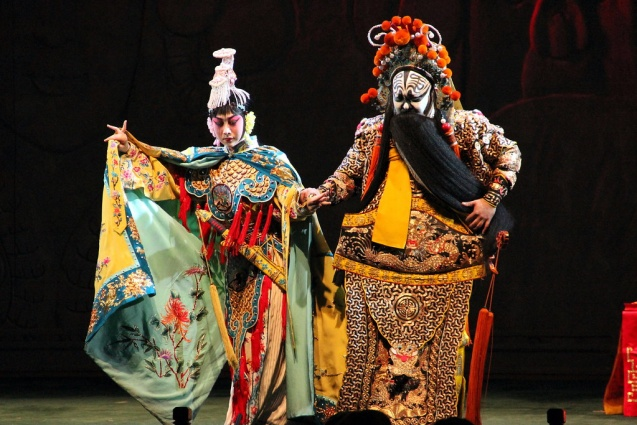
\includegraphics[width=2.88952in,height=1.92917in]{media/image16.jpeg}
%https://openverse.org/image/dd49b785-f3c9-4e76-9a55-70b024eea7c2?q=\%C3\%B3pera\%20de\%20pequim
%Ópera de Beijing - China, Mar2012, Openverse

%Foto: Ana Paula Hirama

( 2 ) O uso de máscaras era uma forte marca desse grupo teatral. Os
espetáculos desse teatro popular aconteciam em palcos improvisados nas
ruas ou praças públicas. Por meio da improvisação, música, figurinos
coloridos, acrobacias, eram apresentadas cenas que ironizavam a vida e
os costumes da época.

%\emph{\textbf{Commedia Dell'Arte}}
%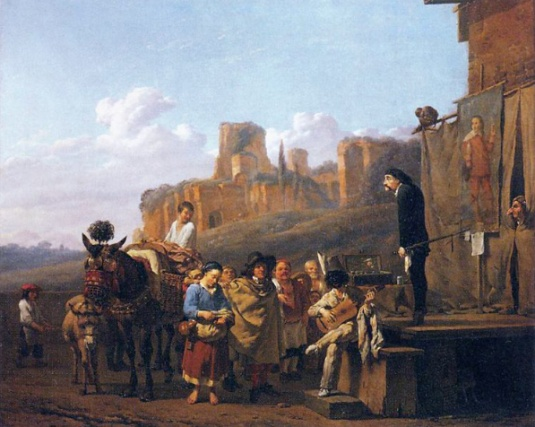
\includegraphics[width=2.43333in,height=1.94028in]{media/image17.jpeg}
%\emph{Os charlatões italianos} (1657), de Karel Dujardins. Óleo sobre tela. 45 x 52 cm. Museu do Louvre, Paris, França.
%\textless{}\href{https://commons.wikimedia.org/wiki/File:Karel_Dujardin_-_Les_Charlatans_italiens.jpg}{\emph{https://commons.wikimedia.org/wiki/File:Karel\_Dujardin\_-\_Les\_Charlatans\_italiens.jpg}}

( 4 ) Criado em Salvador, 1990, esse grupo teatral coloca em prática um
projeto que inclui representar o cotidiano da população negra, sua
religiosidade, o caráter festivo e popular, a dança, os ritmos, os
instrumentos percussivos, a memória ancestral, a estética corporal, as
formas de resistência, a ênfase no registro oral da língua.

%\textbf{Grupo Galpão}
%
\includegraphics[width=2.61458in,height=1.74306in]{media/image18.jpeg}
%https://openverse.org/image/df84bac0-1a9f-48ea-ba22-98c8372b525f?q=grupo\%20galp\%C3\%A3o
%Hoje é dia de estreia do Grupo Galpão na campanha, Openverse

( 3 ) Esse grupo teatral, criado em 1982, é uma companhia brasileira,
originária do teatro popular e de rua. Desenvolvem um teatro resultante
de diversos elementos cênicos e linguagens (circo, farsa, música e
melodrama).

% \textbf{Bando de Teatro Olodum}
%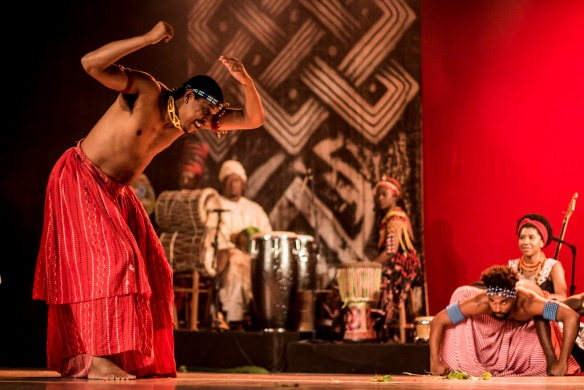
\includegraphics[width=2.65625in,height=1.77170in]{media/image19.jpeg}
%https://openverse.org/image/5c490b9c-2fda-4a5b-98ef-9a63f0d974cc?q=Bando\%20de\%20Teatro\%20Olodum
%Bando de Teatro Olodum, Áfricas - 10/11/2017 - Caixa Cultural Brasília, Openverse

( 1 ) Teatro chinês tradicional surgiu no final do século XVIII. Durante a
atuação, os atores mesclam canto, dança, artes marciais e acrobacias. Em
2010, esse teatro passou a fazer parte do Patrimônio Cultural Imaterial
da Humanidade.

\coment{
Saeb: Analisar o papel dos profissionais e a utilização dos
equipamentos culturais no sistema de produção e circulação das artes
visuais, dança, música e teatro.

Habilidade BNCC: EF69AR24

Respostas na ordem:

2. O uso de máscaras era uma forte marca desse grupo teatral. Os
espetáculos desse teatro popular aconteciam em palcos improvisados nas
ruas ou praças públicas. Por meio da improvisação, música, figurinos
coloridos, acrobacias, eram apresentadas cenas que ironizavam a vida e
os costumes da época;
4. Criado em Salvador, 1990, esse grupo teatral coloca em prática um
projeto que inclui representar o cotidiano da população negra, sua
religiosidade, o caráter festivo e popular, a dança, os ritmos, os
instrumentos percussivos, a memória ancestral, a estética corporal, as
formas de resistência, a ênfase no registro oral da língua;
3. Esse grupo teatral, criado em 1982, é uma companhia brasileira,
originária do teatro popular e de rua. Desenvolvem um teatro resultante
de diversos elementos cênicos e linguagens (circo, farsa, música e
melodrama);
1. Teatro chinês tradicional surgiu no final do século XVIII. Durante a
atuação, os atores mesclam canto, dança, artes marciais e acrobacias. Em
2010, esse teatro passou a fazer parte do Patrimônio Cultural Imaterial
da Humanidade.}

\num{7} Observe a fotografia.

%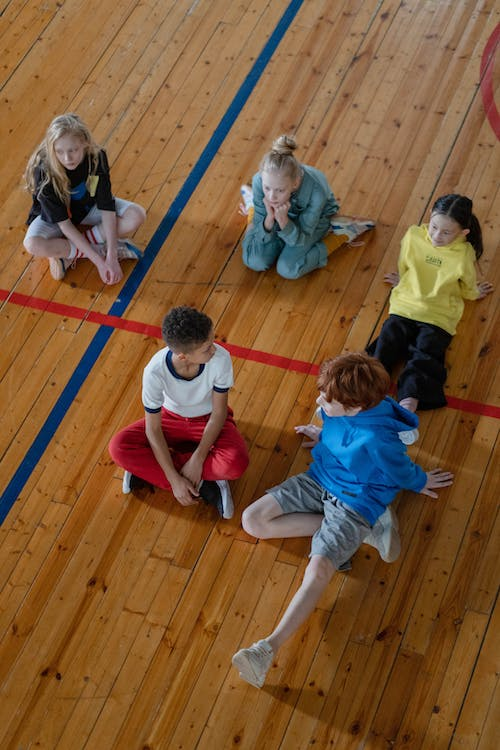
\includegraphics[width=1.72917in,height=2.59375in]{media/image20.jpeg}
%\textless{}https://www.pexels.com/pt-br/foto/cama-leito-quarto-dormitorio-5700174/\textgreater{}

Qual sentimento esse gesto significa?

\linhas{2}
\coment{Resposta pessoal. No entanto, deverão fazer parte da resposta
sentimentos ``negativos'', tais como angústia, ansiedade, aborrecimento,
opressão, desespero, aflição etc.

Saeb: EF69AR10}

\num{8} Leia o texto.

\begin{quote}
\textbf{O que é audiovisual?}

Parece uma pergunta simples. Mas você sabe tudo o que envolve esse tipo
de linguagem? O audiovisual é um meio de comunicação em que há a
utilização conjunta de \textbf{elementos visuais e sonoros}, ou seja,
que pode ser vista e ouvida ao mesmo tempo. Dentre as \textbf{mídias
audiovisuais} destacam-se a
televisão, cinema e vídeos
para a internet. Mas para que a mensagem, som e imagem encontrem a
perfeita harmonia, há uma série de etapas que precisam ser cumpridas,
como: produção; cenografia;
animação; roteiro;
direção de vídeo; edição; figurino; iluminação; fotografia; finalização;
sonorização, entre outros.

\fonte{Disponível em:
https://www.aicinema.com.br/o-que-e-audiovisual. Aceso em: 9 mar. 2023.}
\end{quote}

A partir da leitura do texto, relacione o profissional às suas funções
na produção do audiovisual.

\begin{quote}
1. Diretor\\
2. Design de animação\\
3.  Sonoplasta\\
4. Roteirista
\end{quote}

\begin{boxlist}
\item Cria sequências de imagens e efeitos especiais em 2D ou 3D. \coment{2}

\item Realiza efeitos especiais, fundos sonoros e edita áudio em sincronia com as imagens. \coment{3}

\item Aprova o roteiro, escolhe o elenco, planeja a produção. \coment{1}

\item Cria ou adapta uma narrativa para o audiovisual. \coment{4}
\end{boxlist}

\coment{Saeb: Analisar o papel dos profissionais e a utilização dos
equipamentos culturais no sistema de produção e circulação das artes
visuais, dança, música e teatro.}

Para responder às atividades 9 e 10, leia o texto.

\begin{quote}
\textbf{Por dentro da orquestra}

A orquestra sinfônica atual segue a formação
estabelecida no final do século 18. Dependendo da peça a ser executada,
pode ter mais de 100 instrumentistas. É dividida em quatro famílias
(naipes) de instrumentos:~cordas; madeiras; metais; percussões.

\textbf{Família das cordas}:~É o principal grupo de instrumentos de uma
orquestra. O violino graças à sua versatilidade e alcance, é a principal
voz da família. Divide-se em duas seções: primeiros e segundos violinos.
O~\emph{spalla}, o primeiro violino, comando o conjunto depois do
maestro. Fazem parte dessa família: violino, viola, violoncelo,
contrabaixo e harpa.

\textbf{Família das madeiras}:~Dão ``cor'' ao som da orquestra. A flauta
apesar de ser feita de metal, faz parte da família. Sua variação, o
flautim (ou~\emph{piccolo}) apresenta o som mais agudo entre todos os
instrumentos da orquestra. Fazem parte dessa família: clarinete,
requinta, clarone, flauta,~\emph{picollo}, cornê inglês, oboé, fagote e
contrafagote.

\textbf{Família dos metais}:~Eles são os responsáveis pela avalanche
sonora da orquestra, conferindo a dramaticidade e a grandiosidade que a
obra pede. A trompa e o trompete imprimem agilidade sonora, enquanto o
trombone e a tuba soam de maneira majestosa. Fazem parte dessa família:
trombone, trompete, trompa e tuba.

\textbf{Família das percussões}:~Além de ritmo, os instrumentos de
percussão pontuam e destacam trechos da peça em execução, além de fazer
a orquestra vibrar. Apesar de soar diferente dos outros instrumentos da
família, o piano é considerado percussivo, porque seu som nasce das
batidas dos martelos nas cordas. Fazem parte dessa família: caixa clara,
tímpano, pratos, carrilhão, xilofone, glockenspiel e piano.

\fonte{IMBROISI, Margaret; MARTINS, Simone. Por dentro da Orquestra. História
das Artes, 2023. Disponível em:
https://www.historiadasartes.com/som-camera-acao/musica/os-conjuntos-musicais/.
Acesso em: 09 mar. 2023.}
\end{quote}

\num{9} Entre os parâmetros sonoros, ou seja, as propriedades do som, podemos
citar a duração, a intensidade, a altura e o timbre. Localize no texto e
grife o trecho que aponta um parâmetro de altura.

\linhas{1}
\coment{Trecho: ``apresenta o som mais agudo''.}

\num{10} A seguir, destaque as famílias de instrumentos de uma orquestra e
cite, em cada uma delas, três instrumentos que a compõe.

\linhas{5}
\coment{Família das cordas: violino, viola, violoncelo, contrabaixo e harpa;
família das madeiras: clarinete, requinta, clarone,
flauta,~\emph{picollo}, cornê inglês, oboé, fagote e contrafagote;
família dos metais: trombone, trompete, trompa e tuba; família das
percussões: caixa clara, tímpano, pratos, carrilhão, xilofone,
glockenspiel e piano.}

\coment{
Saeb: Analisar formas, gêneros e estilos distintos de música e teatro
em diferentes contextos, por meio de seus elementos constitutivos.

Habilidade BNCC: EF69AR20 / EF69AR21

Indicamos o vídeo \emph{Instrumentos da orquestra}, que apresenta os
sons produzidos pela maioria dos instrumentos citados no texto.
Disponível em:
https://www.youtube.com/watch?v=lYCE8IqO-tI.
Acesso em: 9 de mar. 2023.

Importante destacar que não há um consenso quanto à classificação da
família do piano. Segundo a maioria dos estudiosos de música, ele
pertence à família de cordas. Para outros, o mecanismo de bater nas
cordas para produzir o som, o classifica como um instrumento de
percussão.}

\colorsec{Treino}

\num{1}  Os triângulos e pratos são instrumentos musicais que fazem parte a
  qual grupo de instrumentos? Marque a alternativa correta.

\begin{escolha}
\item
  Aerofones: instrumentos que produzem som por meio da vibração do ar.
\item
  Cordofones: instrumentos que produzem som por meio da vibração de suas
  cordas.
\item
  Idiofones: instrumentos que produzem som pela própria vibração.
\item
  Membranofones: instrumentos que produzem som pela vibração de uma
  membrana.
\end{escolha}

\coment{
a)  Incorreta. Flauta, trompete e trombone são exemplos de aerofones;
b) Incorreta. Violino, guitarra e harpa são exemplos de cordofones;
c)  Correta. Triângulos, pratos, sinos, produzem som por meio da vibração
  de corpos sólidos, sem estar submetidos a tensão;
d) Incorreta. Surdo, tamborim, pandeiro são exemplos de membrafones.

Saeb: Analisar formas, gêneros e estilos distintos de música e teatro
em diferentes contextos, por meio de seus elementos constitutivos.

BNCC: EF69AR21}

\num{2} Em que período artístico surgiu o balé?

\begin{escolha}
\item Arte na Idade Média (entre século V e XV).

\item Arte Renascentista (por volta do século XIV ao XVII).

\item Arte na Idade Contemporânea (a partir do século XVIII).

\item Arte Moderna (fim do século XIX até meados do XX).
\end{escolha}

\coment{
Resposta:

a) Incorreta. O balé surgiu nas cortes italianas, no início do século XVI;
b) Correta. O balé surgiu na Itália, no início do século XVI, no período renascentista;
c) Incorreta. O balé surgiu nas cortes italianas, no início do século XVI;
d) Incorreta. O balé surgiu nas cortes italianas, no início do século XVI.

Saeb: Analisar o papel dos profissionais e a utilização dos
equipamentos culturais no sistema de produção e circulação das artes
visuais, dança, música e teatro.

BNCC: EF69AR09}

\num{3} Leia o texto.

\begin{quote}
Teatro do Absurdo é uma expressão cunhada pelo crítico húngaro Martin
Esslin (1918-2002) no fim da década de 1950 para abarcar peças que,
surgidas no pós-Segunda Guerra Mundial, tratam da atmosfera de
desolação, solidão e incomunicabilidade do homem moderno por meio de
alguns traços estilísticos e temas que divergem radicalmente da
dramaturgia tradicional realista. Trata-se, porém, não de um movimento
teatral organizado tampouco de um gênero, mas de uma classificação que
visa colocar em destaque uma das tendências teatrais mais importantes da
segunda metade do século XX.

\fonte{Disponível em:
https://enciclopedia.itaucultural.org.br/termo13538/teatro-do-absurdo.
Acesso em: 11 mar. 2023.}
\end{quote}

De acordo com o texto, Teatro do absurdo é

\begin{escolha}
\item
  um gênero teatral que surgiu no fim da década de 1950, no pós-Segunda
  Guerra Mundial.
\item
  um movimento teatral com traços estilísticos e temas que divergem da
  dramaturgia tradicional realista.
\item
  uma classificação que apresenta cenário realista e recriação detalhada
  de uma época ou lugar.
\item
  uma expressão criada para descrever a atmosfera de dor e solidão das
  peças teatrais pós-Segunda Guerra Mundial.
\end{escolha}

\coment{
a)  Incorreta. Não se trata de um gênero teatral;
b)  Incorreta. Não se trata de um movimento teatral;
c)  Incorreta. Cenário realista e recriação detalhada são características
  do teatro tradicional;
d) Correta. É uma expressão cunhada pelo crítico húngaro Martin Esslin,
  para definir os traços estilísticos e temas das peças teatrais no
  pós-Segunda Guerra Mundial.

Saeb: Analisar formas, gêneros e estilos distintos de música e teatro
em diferentes contextos, por meio de seus elementos constitutivos.

BNCC: EF69AR24.}

\chapter{3. Patrimônio cultural, matrizes estéticas e culturais}

\conteudo{\textbf{Patrimônio cultural}

A Constituição da República Federativa do Brasil de 1988 conceitua
patrimônio cultural como sendo

\begin{quote}
os bens de natureza material e imaterial, tomados individualmente ou em
conjunto, portadores de referência à identidade, à ação, à memória dos
diferentes grupos formadores da sociedade brasileira, nos quais se
incluem: as formas de expressão; os modos de criar, fazer e viver; as
criações científicas, artísticas e tecnológicas; as obras, objetos,
documentos, edificações e demais espaços destinados às manifestações
artístico-culturais; os conjuntos urbanos e sítios de valor histórico,
paisagístico, artístico, arqueológico, paleontológico, ecológico e
científico.
\end{quote}

São exemplos de bens culturais materiais, ou seja,
tangíveis (se podem tocar), os que existem numa realidade material
física: cidades, sítios arqueológicos, teatros, igrejas, obras de arte,
vestimentas, documentos, fotografias, áudios e
vídeos.

São exemplos de bens culturais imateriais, ou seja, intangíveis
(não se podem tocar), os que não existem fisicamente ou como uma
realidade material presente o tempo todo: festas, feiras, culinária,
danças, músicas, lendas, crenças populares, rituais e idioma.

\textbf{Matrizes estéticas e culturais}

As principais matrizes brasileiras têm sua origem ou fonte,
inicialmente, nas culturas e estéticas das várias etnias indígenas
(nativos da terra), das variadas etnias de africanos escravizados e dos
europeus (primeiramente os portugueses). Depois, outras culturas e
estéticas foram fazendo parte das nossas matrizes, constituindo assim,
uma identidade e cultura artística própria.

Dessa forma, para que possamos compreender e valorizar os bens culturais
materiais e imateriais do patrimônio brasileiro ou mundial se faz
necessário analisar e avaliar, não somente a própria manifestação
artística ou bem, identificando características sensoriais e artísticas
(estéticas), mas também analisar e avaliar os elementos históricos,
sociais e políticos presentes na origem e no desenvolvimento daquela
arte ao longo do tempo.}

\coment{
Neste módulo, os alunos retomam conteúdos, aprendizagens e experiências
sobre os objetos de conhecimento: patrimônio cultural e matrizes
estéticas e culturais.

Sugerimos que antes da primeira leitura do texto pelos alunos, você
ative os conhecimentos prévios que eles têm sobre o tema, fazendo
algumas perguntas: O que é um patrimônio cultural? O que é um bem
cultural material? Cite exemplos. E o que é bem cultural imaterial? Cite
exemplos. Conhece alguma manifestação artística que tem na sua origem a
cultura africana. Qual? Entre outras possibilidades.

A partir daí, solicite que os alunos leiam o texto, grifando nele as
partes que geraram dúvidas de compreensão do conteúdo, para depois
realizar uma discussão coletiva sobre as informações apresentadas no
texto. Durante a discussão coletiva, intervenha, auxiliando-os na
compreensão das informações contidas no texto.\\
\textbf{Habilidades BNCC}: EF69AR33 / EF69AR34}

\colorsec{Habilidades SAEB}

\begin{quote}
\item Avaliar nas linguagens artísticas a diversidade do patrimônio cultural
da humanidade (material e imaterial), em especial o brasileiro, a partir
de suas diferentes matrizes.

\item Avaliar produções que inter-relacionam diferentes linguagens
artísticas.

\item Avaliar o papel das diversas linguagens artísticas no questionamento
de estereótipos e preconceitos.
\end{quote}

\colorsec{Atividades}

\num{1} Assinale M para bem cultural material e I para bem cultural imaterial.

\begin{boxlist}
\item Igrejas e teatros. \coment{M}

\item Danças e músicas. \coment{I}

\item Crenças populares e festas. \coment{I}

\item Áudios e vídeos. \coment{M}
\end{boxlist}

\coment{
Saeb: Avaliar nas linguagens artísticas a diversidade do patrimônio
cultural da humanidade (material e imaterial), em especial o brasileiro,
a partir de suas diferentes matrizes.

Habilidade BNCC: EF69AR34}

\num{2}  Leia o texto.

\begin{quote}
O documento \emph{Convenção para a Salvaguarda do Patrimônio Cultural
Imaterial}, publicado pela UNESCO, Paris, 17 de outubro de 2003, assim
define o patrimônio cultural imaterial:

Entende-se por ``patrimônio cultural imaterial'' as práticas,
representações, expressões, conhecimentos e técnicas - junto com os
instrumentos, objetos, artefatos e lugares culturais que lhes são
associados - que as comunidades, os grupos e, em alguns casos, os
indivíduos reconhecem como parte integrante de seu patrimônio cultural.
Este patrimônio cultural imaterial, que se transmite de geração em
geração, é constantemente recriado pelas comunidades e grupos em função
de seu ambiente, de sua interação com a natureza e de sua história,
gerando um sentimento de identidade e continuidade e contribuindo assim
para promover o respeito à diversidade cultural e à criatividade humana.

\fonte{Disponível em:
https://unesdoc.unesco.org/ark:/48223/pf0000132540_por. Acesso em:
14 mar. 2023.}
\end{quote}

Escolha um campo de manifestação e cite um patrimônio cultural imaterial
de sua comunidade que deve ser salvaguardado (protegido, conservado,
preservado) e justifique sua resposta.

\textbf{Campos de manifestação}:

\begin{escolha}
\item
  Tradições e expressões orais;
\item
  Expressões artísticas;
\item
  Práticas sociais, rituais e atos festivos;
\item
  Conhecimentos e práticas relacionados à natureza e ao universo;
\item
  Técnicas artesanais.
\end{escolha}

\linhas{5}
\coment{Resposta pessoal.}

\coment{
Saeb: Avaliar nas linguagens artísticas a diversidade do patrimônio
cultural da humanidade (material e imaterial), em especial o brasileiro,
a partir de suas diferentes matrizes.

Habilidade BNCC: EF69AR34}

Para responder às atividades 3 a 5, leia o texto.

\begin{quote}
A~Literatura de Cordel no Brasil é o resultado de uma série de
práticas culturais em que os cantos e os contos -- e suas variantes --
constituem as matrizes a partir das quais uma série de formas de
expressão se forjou. Na formação da cultura brasileira, da qual a
literatura de cordel faz parte, tanto indígenas quanto africanos e
portugueses adicionaram práticas de transmissão oral de suas
cosmologias, de seus contos, de suas canções.~A questão da harmonia
sonora é muito ressaltada pelos poetas. Além das razões estéticas, há
uma explicação histórica para isso. No início do século XX, quando a
literatura de cordel se consolidou como um sistema editorial próprio, os
poetas desenvolveram um modo particular de comercializar seus livros nos
mercados e feiras livres. Carregavam consigo os exemplares e montavam
uma banca em que os folhetos eram exibidos. Para atrair curiosos e
compradores, os poetas costumavam cantar em voz alta trechos dos poemas,
contando dramas, tragédias, romances e sátiras. No momento mais
importante da narrativa -- quando o desfecho da história de aproximava
-- o canto era interrompido e o final da história só poderia ser
conhecido por aqueles que comprassem o folheto. Assim, a métrica
perfeita era a condição para que o poeta pudesse exercer sua performance
com maestria diante do público.

\fonte{Disponível em: http://portal.iphan.gov.br/noticias/detalhes/4819. Acesso
em: 13 mar. 2023.}
\end{quote}

\num{1}  Quais são as matrizes culturais da Literatura de Cordel?

\linhas{2}
\coment{A Literatura de Cordel recebeu contribuições das culturas africana,
indígena e europeia (portugueses).

Saeb: Avaliar nas linguagens artísticas a diversidade do patrimônio
cultural da humanidade (material e imaterial), em especial o brasileiro,
a partir de suas diferentes matrizes.

Habilidade BNCC: EF69AR34}

\num{2}  Com base no texto que você leu, assinale V para verdadeiro e F para falso.

\begin{boxlist}
\item A Literatura de Cordel era vendida em mercados e feiras livres, desde sua origem.\coment{F}
\item A Literatura de Cordel é um patrimônio cultural material.\coment{F}
\item A Literatura de cordel é um patrimônio cultural imaterial.\coment{V}
\item A Literatura de Cordel é uma forma de expressão da literatura tradicional.\coment{F}
\end{boxlist}

\coment{
Saeb: Avaliar nas linguagens artísticas a diversidade do patrimônio
cultural da humanidade (material e imaterial), em especial o brasileiro,
a partir de suas diferentes matrizes.

Habilidade BNCC: EF69AR34}

\num{3} Marque, no texto, o trecho que explica uma prática histórica utilizada
  pelos cordelistas para a divulgação e a comercialização da Literatura
  de Cordel.

\coment{
Trecho: No início do século XX, quando a literatura de cordel se
consolidou como um sistema editorial próprio, os poetas desenvolveram um
modo particular de comercializar seus livros nos mercados e feiras
livres. Carregavam consigo os exemplares e montavam uma banca em que os
folhetos eram exibidos. Para atrair curiosos e compradores, os poetas
costumavam cantar em voz alta trechos dos poemas, contando dramas,
tragédias, romances e sátiras. No momento mais importante da narrativa
-- quando o desfecho da história de aproximava -- o canto era
interrompido e o final da história só poderia ser conhecido por aqueles
que comprassem o folheto.

Saeb: Avaliar nas linguagens artísticas a diversidade do patrimônio
cultural da humanidade (material e imaterial), em especial o brasileiro,
a partir de suas diferentes matrizes.

Habilidade BNCC: EF69AR34}

Para responder às atividades 6 e 7, leia o texto.

%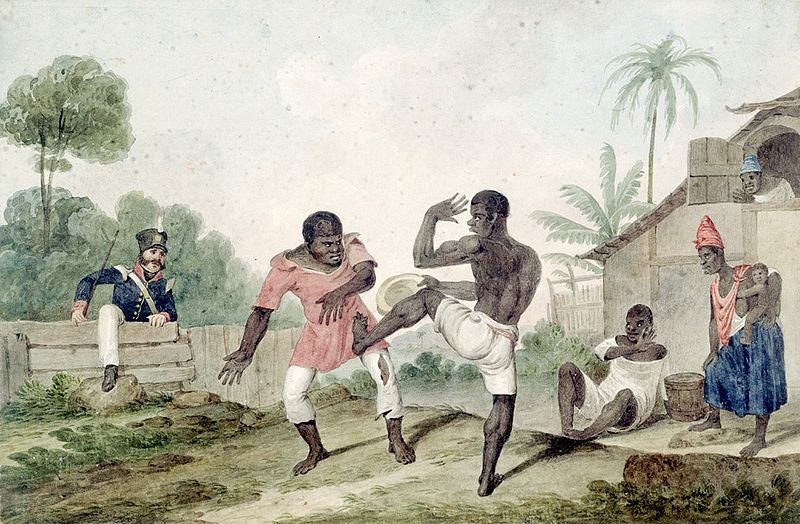
\includegraphics[width=2.77083in,height=1.81490in]{media/image21.jpeg}
%Pintura de Augustus Earle representando o ``jogo ilegal de capoeira'', em 1824, no Rio de Janeiro.
%https://commons.wikimedia.org/wiki/File:CapoeiraEarle.JPG

\begin{quote}
\textbf{Patrimônio Cultural Imaterial da Humanidade}\\
 A~9ª Sessão do
Comitê Intergovernamental para a Salvaguarda aprovou, em novembro de
2014, em Paris, a Roda de Capoeira, um dos símbolos do Brasil mais
reconhecidos internacionalmente, como Patrimônio Cultural Imaterial da
Humanidade. O reconhecimento da Roda de Capoeira, pela Unesco, é uma
conquista muito importante para a cultura brasileira e expressa a
história de resistência negra no Brasil, durante e após a
escravidão.~Originada no século XVII, em pleno período escravista,
desenvolveu-se como forma de sociabilidade e solidariedade entre os
africanos escravizados, estratégia para lidarem com o controle e a
violência. Hoje, é um dos maiores símbolos da identidade brasileira e
está presente em todo território nacional, além de praticada em mais de
160 países, em todos os continentes.

\fonte{Disponível em: http://portal.iphan.gov.br/pagina/detalhes/66.
Acesso em: 13 mar. 2023.}
\end{quote}

\begin{enumerate}
\def\labelenumi{\arabic{enumi}.}
\setcounter{enumi}{2}
\item
  Mesmo após a abolição da escravatura, a prática da capoeira continuou
  sendo vista como subversiva e apenas em 1937 deixou de ser considerada
  criminosa pelo Código Penal brasileiro. Destaque no texto a informação
  que reforça essa afirmativa.
\end{enumerate}

Deve ser destacado o texto ``jogo ilegal da capoeira'', presente na
legenda da imagem.

\coment{
Saeb: - Avaliar produções que inter-relacionam diferentes linguagens
artísticas.

Habilidade EF69AR33: Analisar aspectos históricos, sociais e políticos
da produção artística, problematizando as narrativas eurocêntricas e as
diversas categorizações da arte (arte, artesanato, folclore, design
etc.).

\begin{enumerate}
\def\labelenumi{\arabic{enumi}.}
\setcounter{enumi}{2}
\item
  Em qual período histórico, social e político surgiu a Roda de
  Capoeira?
\end{enumerate}

Surgiu no século XVII, período colonial brasileiro.

\coment{
Saeb: - Avaliar produções que inter-relacionam diferentes linguagens
artísticas.

Habilidade EF69AR33: Analisar aspectos históricos, sociais e políticos
da produção artística, problematizando as narrativas eurocêntricas e as
diversas categorizações da arte (arte, artesanato, folclore, design
etc.).

\begin{enumerate}
\def\labelenumi{\arabic{enumi}.}
\setcounter{enumi}{2}
\item
  Relacione os patrimônios imateriais com seus respectivos livros de
  registro no Instituto do Patrimônio Histórico e Artístico Nacional
  (IPHAN), tendo como base a descrição do conteúdo dos livros de
  registro.
\end{enumerate}

\begin{longtable}[]{@{}lll@{}}
\toprule
\begin{minipage}[b]{0.32\columnwidth}\raggedright\strut
\begin{enumerate}
\def\labelenumi{\arabic{enumi}.}
\item
  \textbf{Frevo}
\end{enumerate}

\textless{}https://commons.wikimedia.org/wiki/File:Munguz\%C3\%A1\_de\_Zuza\_Miranda\_\%26\_Thais,\_e\_Bacalhau\_do\_Batata\_-\_Carnaval\_2013\_(8496877781).jpg?uselang=pt\textgreater{}\strut
\end{minipage} & \begin{minipage}[b]{0.32\columnwidth}\raggedright\strut
\strut
\end{minipage} & \begin{minipage}[b]{0.32\columnwidth}\raggedright\strut
( 3 ) \textbf{Livro de Registro das~Celebrações}~-Reúne os rituais e
festas que marcam vivência coletiva, religiosidade, entretenimento e
outras práticas da vida social, que marcam a vivência coletiva de um
grupo social, sendo considerados importantes para a sua cultura, memória
e identidade,~e acontecem em lugares ou territórios específicos.\strut
\end{minipage}\tabularnewline
\midrule
\endhead
\begin{minipage}[t]{0.32\columnwidth}\raggedright\strut
\begin{enumerate}
\def\labelenumi{\arabic{enumi}.}
\item
  \textbf{Ofício das Baianas de Acarajé}
\end{enumerate}

\textless{}\url{https://openverse.org/image/aad5dfe0-37eb-46c6-a58f-b84ee26425c6?q=baiana\%20do\%20acaraj\%C3\%A9}\textgreater{}\strut
\end{minipage} & \begin{minipage}[t]{0.32\columnwidth}\raggedright\strut
\strut
\end{minipage} & \begin{minipage}[t]{0.32\columnwidth}\raggedright\strut
~( 4 ) \textbf{Livro de Registro dos Lugares}~- Nele são~inscritos os
lugares que possuem sentido cultural diferenciado para a população
local, onde são realizadas práticas e atividades de naturezas variadas,
tanto cotidianas quanto excepcionais, tanto vernáculas (próprias do país
ou região) quanto oficiais.\strut
\end{minipage}\tabularnewline
\begin{minipage}[t]{0.32\columnwidth}\raggedright\strut
\begin{enumerate}
\def\labelenumi{\arabic{enumi}.}
\item
  \textbf{Complexo Cultural do Boi Bumbá do Médio Amazonas e Parintins}
\end{enumerate}

Festival de Parintins

\textless{}https://openverse.org/image/d732f0da-eab6-4435-9bfa-2e5d57d4bef1?q=Boi\%20Bumb\%C3\%A1\textgreater{}\strut
\end{minipage} & \begin{minipage}[t]{0.32\columnwidth}\raggedright\strut
\strut
\end{minipage} & \begin{minipage}[t]{0.32\columnwidth}\raggedright\strut
( 1 ) \textbf{Livro de Registro~das Formas de Expressão}~- Formas de
Expressão são formas de comunicação associadas a determinado grupo
social ou região, desenvolvidas por atores sociais reconhecidos pela
comunidade e em relação às quais o costume define normas, expectativas e
padrões de qualidade. Trata-se da apreensão das performances culturais
de grupos sociais, como manifestações literárias, musicais, plásticas,
cênicas e lúdicas, que são por eles consideradas importantes para a sua
cultura, memória e identidade.\strut
\end{minipage}\tabularnewline
\begin{minipage}[t]{0.32\columnwidth}\raggedright\strut
\begin{enumerate}
\def\labelenumi{\arabic{enumi}.}
\item
  \textbf{Feira de Caruaru}
\end{enumerate}

Feira de Caruaru, Pernambuco.

\textless{}https://www.flickr.com/photos/allanpatrick/330960263/\textgreater{}\strut
\end{minipage} & \begin{minipage}[t]{0.32\columnwidth}\raggedright\strut
\strut
\end{minipage} & \begin{minipage}[t]{0.32\columnwidth}\raggedright\strut
( 2 ) \textbf{Livro de Registro dos Saberes} --

Os\textbf{~}Saberes~são conhecimentos tradicionais associados a
atividades desenvolvidas por atores sociais reconhecidos como grandes
conhecedores de técnicas, ofícios e matérias-primas que identifiquem um
grupo social ou uma localidade. Geralmente estão associados à produção
de objetos e/ou prestação de serviços~que podem ter sentidos práticos ou
rituais.\strut
\end{minipage}\tabularnewline
\bottomrule
\end{longtable}

Disponível em: \url{http://portal.iphan.gov.br/pagina/detalhes/122}.
Acesso em: 13 mar. 2023. (Adaptado para fins didáticos)

\coment{
Saeb: - Avaliar nas linguagens artísticas a diversidade do patrimônio
cultural da humanidade (material e imaterial), em especial o brasileiro,
a partir de suas diferentes matrizes.

Habilidade: EF69AR34

Para responder às atividades 9 e 10, leia o texto.

O patrimônio pode ser classificado por duas grandes divisões: natureza e
cultura. Patrimônio natural são as riquezas que estão no solo e subsolo,
tanto as florestas quanto jazidas. O conceito de patrimônio cultural vem
sendo ampliado à medida que se revisa o conceito de cultura. Atualmente,
há consenso de que a noção de patrimônio cultural é muito mais ampla.
Não inclui apenas os bens tangíveis, como também os intangíveis, não só
as manifestações artísticas, mas todo o fazer humano, e não só aquilo
que representa a cultura das classes mais abastadas, mas o que
representa a cultura dos menos favorecidos.

Nesse sentido, o patrimônio deixou de ser definido pelos prédios que
abrigaram reis, condes e marqueses e pelos utensílios a eles
pertencentes. Passou a ser definido como o conjunto de todos os
utensílios, hábitos, usos e costumes, crenças e forma de vida cotidiana
de todos os segmentos que compuseram e compõem a sociedade ao longo dos
anos.

Disponível em:
\url{https://bdm.unb.br/bitstream/10483/385/1/2004_JaniceDelFrariCoutinho.pdf}.
Acesso em 14 mar. 2023.

\begin{enumerate}
\def\labelenumi{\arabic{enumi}.}
\setcounter{enumi}{2}
\item
  De acordo com o texto, o que era considerado patrimônio cultural na
  visão tradicional, eurocêntrica (tendência a interpretar o mundo
  segundo os valores do ocidente europeu)?
\end{enumerate}

Os bens que representavam a cultura das classes mais abastadas.

\coment{
Saeb: - Avaliar o papel das diversas linguagens artísticas no
questionamento de estereótipos e preconceitos.

BNCC: EF69AR33

\begin{enumerate}
\def\labelenumi{\arabic{enumi}.}
\setcounter{enumi}{2}
\item
  De acordo com o texto, o que é considerado patrimônio cultural na
  atualidade?
\end{enumerate}

Na atualidade, são considerados como patrimônio cultural o conjunto de
todos os utensílios, hábitos, usos e costumes, crenças e forma de vida
cotidiana de todos os segmentos que compuseram e compõem a sociedade ao
longo dos anos.

\coment{
Saeb: - Avaliar o papel das diversas linguagens artísticas no
questionamento de estereótipos e preconceitos.

BNCC: EF69AR33

.

\colorsec{Treino}

\begin{enumerate}
\def\labelenumi{\arabic{enumi}.}
\item
  Entre os patrimônios imateriais listados a seguir, qual pode ser
  descrito como patrimônio ``onde se expressam simultaneamente o canto,
  o toque dos instrumentos, a dança, os golpes, o jogo, a brincadeira,
  os símbolos e rituais de herança africana - notadamente banto -
  recriados no Brasil.'' (IPHAN)
\end{enumerate}

\begin{quote}
(http://portal.iphan.gov.br/pagina/detalhes/66)
\end{quote}

a. Carimbó.

b. Frevo.

c. Samba de Roda do Recôncavo Baiano

d. Roda de capoeira.

\coment{
Resposta:

\begin{enumerate}
\def\labelenumi{\Alph{enumi}.}
\item
  \begin{quote}
  Incorreta. O Carimbó expressa o canto, o toque dos instrumentos e a
  dança, com influências culturais indígena, africana e europeia. Os
  outros elementos são característicos da Roda de Capoeira.
  \end{quote}
\item
  \begin{quote}
  Incorreta. O Frevo é uma forma de expressão musical, coreográfica e
  poética, originária em Pernambuco. Os outros elementos são
  característicos da Roda de Capoeira.
  \end{quote}
\item
  \begin{quote}
  Incorreta. O Samba de Roda do Recôncavo Baiano é uma expressão
  musical, coreográfica, poética e festiva, com matrizes africana e
  europeia.
  \end{quote}
\item
  \begin{quote}
  Correta.
  \end{quote}
\end{enumerate}

Saeb: - Avaliar produções que inter-relacionam diferentes linguagens
artísticas.

BNCC: EF69AR34

\begin{enumerate}
\def\labelenumi{\arabic{enumi}.}
\item
  Leia o texto.
\end{enumerate}

Os processos de globalização e de transformação social, ao mesmo tempo
em que criam condições propícias para um diálogo renovado entre as
comunidades, geram também, da mesma forma que o fenômeno da
intolerância, graves riscos de deterioração, desaparecimento e
destruição do patrimônio cultural imaterial, devido em particular à
falta de meios para sua salvaguarda.

Disponível em:
\url{https://unesdoc.unesco.org/ark:/48223/pf0000132540_por}. Acesso em:
14 mar. 2023.

Cada alternativa contém um depoimento retirado de uma notícia divulgada
no Brasil. Assinale a alternativa que apresenta o fenômeno da
intolerância, graves riscos de deterioração, desaparecimento e
destruição do patrimônio cultural imaterial.

\begin{enumerate}
\def\labelenumi{\alph{enumi}.}
\item
  ``Foi lamentável a imagem da escultura do meu avô, Ariano, no chão, um
  ato de depreciação do patrimônio público e até de nossa cultura''.
\end{enumerate}

Disponível em:
\url{https://g1.globo.com/pe/pernambuco/noticia/2020/09/22/depreciacao-do-patrimonio-publico-e-ate-de-nossa-cultura-diz-neta-de-ariano-suassuna-sobre-escultura-depredada-no-recife.ghtml}.
Acesso em: 14 mar. 2023.

\begin{enumerate}
\def\labelenumi{\alph{enumi}.}
\item
  "Nem mesmo as obras que valorizam a nossa cultura foram poupadas. Nove
  monumentos e diversos brasões, principalmente nas pontes e no Bairro
  do Recife, também sofreram ações de depredação e furtos, somando um
  prejuízo de quase R\$ 400 mil, que só não foi maior porque algumas
  peças foram resgatadas".
\end{enumerate}

Disponível em:
\url{https://www.diariodepernambuco.com.br/noticia/vidaurbana/2023/01/vandalismo-e-furtos-de-patrimonio-publico-causaram-prejuizos-de-r-2-4.html}.
Acesso em: 14 mar. 2023.

\begin{enumerate}
\def\labelenumi{\alph{enumi}.}
\item
  ``Hoje estamos todos juntos comemorando, vestidos de branco, pedindo
  paz e respeito para a nossa religião. Estamos reivindicando um direito
  que já é nosso e está escrito na Constituição mas, infelizmente, não
  funciona assim''.
\end{enumerate}

Disponível em:
https://www.correio24horas.com.br/noticia/nid/povo-do-axe-vai-as-ruas-pelo-fim-da-intolerancia-religiosa.
Acesso em: 14 mar. 2023.

\begin{enumerate}
\def\labelenumi{\alph{enumi}.}
\item
  ``A gestão municipal gasta muito para recuperar espaços e apagar
  pichações praticamente todos os dias''. E completou: ``O custo e o
  dano desses atos de vandalismo infelizmente vêm para a própria
  população, pois deixamos de fazer novas obras, para recuperar
  outras''.
\end{enumerate}

Disponível em:
\url{https://www.correio24horas.com.br/noticia/nid/monumento-cleriston-andrade-e-pichado-mais-uma-vez}.
Acesso em: 14 mar. 2023.

\coment{
Resposta:

\begin{enumerate}
\def\labelenumi{\alph{enumi}.}
\item
  Incorreta. Escultura é um patrimônio cultural imaterial.
\item
  Incorreta. Monumentos fazem parte do patrimônio cultural material.
\item
  Correta. Cultos e religiões fazem parte do patrimônio cultural
  imaterial.
\item
  Incorreta. Pichações em espaços físicos do município, patrimônios
  culturais materiais.
\end{enumerate}

Saeb: - Avaliar o papel das diversas linguagens artísticas no
questionamento de estereótipos e preconceitos.

BNCC: EF69AR34

\begin{enumerate}
\def\labelenumi{\arabic{enumi}.}
\item
  Leia o texto.
\end{enumerate}

\begin{longtable}[]{@{}ll@{}}
\toprule
\begin{minipage}[t]{0.48\columnwidth}\raggedright\strut
Igreja São Francisco de Assis, Belo Horizonte.

\textless{}
\url{http://openverse.org/image/fa3dde90-6c73-4d4f-a966-5d4c4a4f6685?q=Igreja\%20de\%20São\%20Francisco\%20de\%20Assis\%20belo\%20horizonte}\textgreater{}\strut
\end{minipage} & \begin{minipage}[t]{0.48\columnwidth}\raggedright\strut
O Conjunto Moderno da Pampulha, situado em uma das regiões mais
tradicionais de Belo Horizonte (MG), recebeu o título de Patrimônio
Mundial, no dia 16 de julho de 2016.

Formado por quatro edifícios articulados em torno do espelho d'água de
um lago urbano artificial, é composto pela Igreja de São Francisco de
Assis, o Cassino (atual Museu de Arte da Pampulha), a Casa do Baile
(Centro de Referência em Urbanismo, Arquitetura e Design de Belo
Horizonte) e o Iate Golfe Clube (Iate Tênis Clube), bens construídos
entre 1942 e 1943. Completam esse patrimônio cultural os painéis em
azulejos criados por Candido Portinari, esculturas de artistas renomados
como Alfredo Ceschiatti e José Alves Pedrosa, e os jardins planejados
pelo paisagista Roberto Burle Marx.\strut
\end{minipage}\tabularnewline
\bottomrule
\end{longtable}

Disponível em \url{http://portal.iphan.gov.br/pagina/detalhes/820}.
Acesso em: 14 mar. 2023. (Texto adaptado para fins didáticos.)

Segundo sua natureza, como pode ser classificado o \emph{Conjunto
Moderno da Pampulha}? Assinale a alternativa correta.

\begin{enumerate}
\def\labelenumi{\alph{enumi}.}
\item
  Patrimônio arqueológico.
\item
  Patrimônio paisagístico.
\item
  Patrimônio etnográfico.
\item
  Patrimônio das artes aplicadas.
\end{enumerate}

\coment{
Resposta:

\begin{enumerate}
\def\labelenumi{\alph{enumi}.}
\item
  Incorreta. Fazem parte do patrimônio arqueológico os bens relacionados
  a vestígios da ocupação pré-histórica.
\item
  Correta. Fazem parte do patrimônio paisagístico tanto as áreas
  naturais, quanto lugares criados pelo homem aos quais é atribuído
  valor à sua configuração paisagística e que se destaquem por sua
  relação com o território onde se encontram.
\item
  Incorreta. Fazem parte do patrimônio etnográfico bens de valor
  etnográfico e de referência para grupos sociais.
\item
  Incorreta. Fazem parte do patrimônio das artes aplicadas os bens que
  têm seu valor artístico associado à função utilitária, muito comum na
  arquitetura, design e artes gráficas.
\end{enumerate}

Saeb: - Avaliar nas linguagens artísticas a diversidade do patrimônio
cultural da humanidade (material e imaterial), em especial o brasileiro,
a partir de suas diferentes matrizes.

BNCC: EF69AR33

\textbf{Simulados -- 9º ano -- Arte}

\textbf{Simulado 1}

\begin{enumerate}
\def\labelenumi{\arabic{enumi}.}
\item
  Observe a pintura.
\end{enumerate}

\begin{quote}
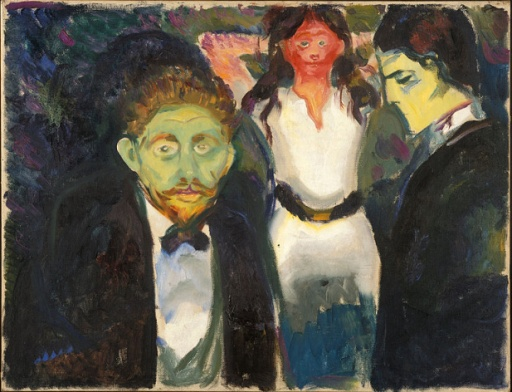
\includegraphics[width=2.62500in,height=2.00000in]{media/image27.jpeg}
\end{quote}

\emph{Inveja},1907, de Edvard Munch. Óleo sobre tela, 75 cm x 98 cm.
Museu Munch, Oslo, Noruega.

\emph{\textless{}}\url{https://commons.wikimedia.org/wiki/File:Edvard_Munch_-_Jealousy_-_Google_Art_Project.jpg}\emph{\textgreater{}}

Esta imagem é a reprodução de uma pintura

\begin{enumerate}
\def\labelenumi{\alph{enumi})}
\item
  impressionista.
\item
  cubista.
\item
  expressionista.
\item
  surrealista.
\end{enumerate}

Nível: difícil.

\begin{enumerate}
\def\labelenumi{\alph{enumi})}
\item
  Incorreta. A pintura impressionista, aproveita ao máximo a
  luminosidade e é marcada por pinceladas soltas, buscando o registro da
  experiência contemporânea.
\item
  Incorreta. A pintura cubista é caracterizada pela recusa à ideia da
  arte como imitação da natureza e pelas formas geométricas.
\item
  Correta. A pintura expressionista reforça a distorção das formas da
  realidade, por meio do alto contraste de cores, em busca da
  subjetividade da expressão.
\item
  Incorreta. A pintura surrealista buscava no subconsciente e sonhos sua
  inspiração, criando uma realidade paralela.
\end{enumerate}

Saeb: - Analisar formas, gêneros e estilos distintos de artes visuais e
dança, em diferentes contextos, por meio de seus elementos
constitutivos.

BNCC: (EF69AR01) Pesquisar, apreciar e analisar formas distintas das
artes visuais tradicionais e contemporâneas, em obras de artistas
brasileiros e estrangeiros de diferentes épocas e em diferentes matrizes
estéticas e culturais, de modo a ampliar a experiência com diferentes
contextos e práticas artístico-visuais e cultivar a percepção, o
imaginário, a capacidade de simbolizar e o repertório imagético.

\begin{enumerate}
\def\labelenumi{\arabic{enumi}.}
\item
  Observe a pintura.
\end{enumerate}

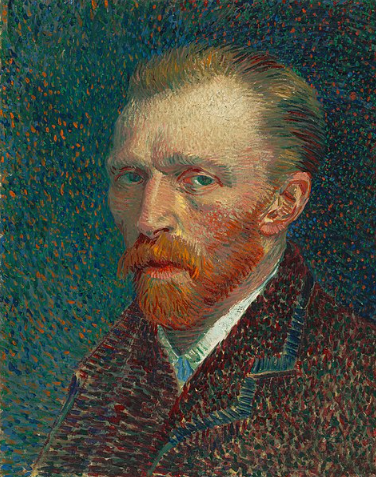
\includegraphics[width=3.16667in,height=4.01042in]{media/image28.png}

Vincent van Gogh.

\textless{}
https://commons.wikimedia.org/wiki/File:Vincent\_van\_Gogh\_-\_Self-Portrait\_-\_Google\_Art\_Project\_(454045).jpg\textgreater{}

Produzida em 1887, a pintura pertence a qual gênero da arte visual?
Marque a alternativa correta.

\begin{enumerate}
\def\labelenumi{\alph{enumi})}
\item
  Autorretrato.
\item
  Natureza-morta.
\item
  Paisagem.
\item
  Retrato.
\end{enumerate}

Nível: fácil.

\begin{enumerate}
\def\labelenumi{\alph{enumi})}
\item
  Correta. O pintor Vincent Van Gogh retratou a si mesmo nessa obra.
\item
  Incorreta. O gênero natureza-morta refere-se à representação de
  objetos inanimados.
\item
  Incorreta. O gênero paisagem refere-se à representação de um local.
\item
  Incorreta. O gênero retrato refere-se à representação de uma figura
  individual ou de um grupo.
\end{enumerate}

Saeb: - Analisar formas, gêneros e estilos distintos de artes visuais e
dança, em diferentes contextos, por meio de seus elementos
constitutivos.

BNCC: (EF69AR01) Pesquisar, apreciar e analisar formas distintas das
artes visuais tradicionais e contemporâneas, em obras de artistas
brasileiros e estrangeiros de diferentes épocas e em diferentes matrizes
estéticas e culturais, de modo a ampliar a experiência com diferentes
contextos e práticas artístico-visuais e cultivar a percepção, o
imaginário, a capacidade de simbolizar e o repertório imagético.

\begin{enumerate}
\def\labelenumi{\arabic{enumi}.}
\item
  Observe a imagem e leia o texto.
\end{enumerate}

\begin{longtable}[]{@{}ll@{}}
\toprule
\begin{minipage}[t]{0.48\columnwidth}\raggedright\strut
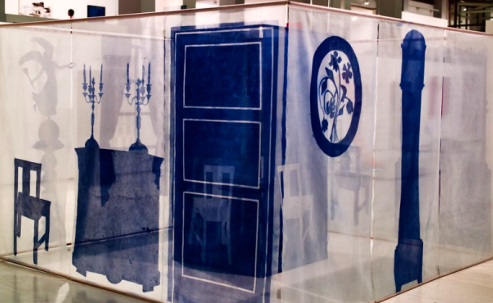
\includegraphics[width=2.23958in,height=1.37500in]{media/image29.png}

\emph{Ambiente - Sala de jantar} (1971), Ana Vieira. Museu Calouste
Gulbenkian, Coleção Moderna, Lisboa, Portugal.

\textless{}\href{https://www.flickr.com/photos/pedrosimoes7/49086771662/in/photolist-2hMCx4m-FxMXcX-QAvunL-FHPfUJ-JHyVGM-FyWhZ5-D9e7EX-FNocrk-qqG1VK-2jorxjG-2jo51A9-2iogqpn-2f1XQVG-2j1SNKo-2iWC9hZ-2iohmHT-ERRvQ7-2iJusb2-2iSKWtb-2gzpG4G-SXqY31-4axCty-RvGFdh-RvGFjj-RvGFgU-4cLsjY-5mSoVV-8RSQ7A-4a1HDm-4an2jV-4atvMR-4atvzp-KwqJ6X-4atvxD-4atvHV-4atvKz-4atvDH-K6ioNh-K6iwq1-JA2Qvi-K6ioQS-JzT7Zu-JzSgg1-KpuVmn-KpuVfR-KtwQpf-JzS8jQ-KmYaQ7-KpuVwH-KpuURV}{\emph{https://www.flickr.com/photos/pedrosimoes7/49086771662/in/photolist-2hMCx4m-FxMXcX-QAvunL-FHPfUJ-JHyVGM-FyWhZ5-D9e7EX-FNocrk-qqG1VK-2jorxjG-2jo51A9-2iogqpn-2f1XQVG-2j1SNKo-2iWC9hZ-2iohmHT-ERRvQ7-2iJusb2-2iSKWtb-2gzpG4G-SXqY31-4axCty-RvGFdh-RvGFjj-RvGFgU-4cLsjY-5mSoVV-8RSQ7A-4a1HDm-4an2jV-4atvMR-4atvzp-KwqJ6X-4atvxD-4atvHV-4atvKz-4atvDH-K6ioNh-K6iwq1-JA2Qvi-K6ioQS-JzT7Zu-JzSgg1-KpuVmn-KpuVfR-KtwQpf-JzS8jQ-KmYaQ7-KpuVwH-KpuURV}}\textgreater{}\strut
\end{minipage} & \begin{minipage}[t]{0.48\columnwidth}\raggedright\strut
A instalação \emph{Ambiente - Sala de jantar} expõe entre paredes de
nylon pinturas, com spray azul, de objetos e móveis. No espaço interno,
encontra-se uma mesa posta com pratos de louça, copos de vidro, garfos e
facas em inox, associada a uma gravação de áudio com as sonoridades
próprias de uma refeição: diálogo entre pessoas e ruído de talheres e
pratos, com foco de luz incidente sobre a mesa.\strut
\end{minipage}\tabularnewline
\bottomrule
\end{longtable}

A escolha do tema ``Ambiente de uma sala de jantar'' permitiu que a
artista portuguesa, Ana Vieira, integrasse diferentes linguagens
artísticas. Assinale a alternativa que contém duas fontes materiais
utilizadas na obra.

\begin{enumerate}
\def\labelenumi{\alph{enumi})}
\item
  Espaço e gesto.
\item
  Instrumento musical e tinta spray.
\item
  Luz e som.
\item
  Pincel e som.
\end{enumerate}

Nível: médio.

\begin{enumerate}
\def\labelenumi{\alph{enumi})}
\item
  Incorreta. Segundo a descrição do texto, a artista não utilizou o
  gesto.
\item
  Incorreta. Segundo a descrição do texto, a artista não utilizou
  instrumento musical.
\item
  Correta. Luz e som são materialidades presentes na obra.
\item
  Incorreta. Segundo a descrição do texto, a artista não utilizou
  pincel.
\end{enumerate}

Saeb: - Analisar a função do tema como projeto integrador das diferentes
linguagens artísticas.

BNCC: (EF69AR03) Analisar situações nas quais as linguagens das artes
visuais se integram às linguagens audiovisuais (cinema, animações,
vídeos etc.), gráficas (capas de livros, ilustrações de textos diversos
etc.), cenográficas, coreográficas, musicais etc.

\textbf{Simulado 2}

\begin{enumerate}
\def\labelenumi{\arabic{enumi}.}
\item
  Observe a imagem.
\end{enumerate}

\textbf{\textless{}Editora, desenhar a árvore do Teatro do Oprimido
tendo como base a imagem a seguir. Importante, destacar o solo, com cor
de fundo diferenciada.\textgreater{}}

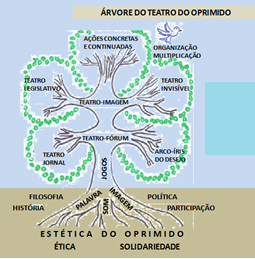
\includegraphics[width=2.65625in,height=2.69792in]{media/image30.png}

Augusto Boal, diretor de teatro, dramaturgo e ensaísta brasileiro,
escolheu a árvore para representar a metodologia do Teatro do Oprimido.
No~\textbf{solo} encontra-se a representação:

\begin{enumerate}
\def\labelenumi{\alph{enumi})}
\item
  das técnicas desenvolvidas pelo Teatro do Oprimido.
\item
  das técnicas consideradas como base do método.
\item
  das ações necessárias para a transformação social.
\item
  do conjunto de saberes acumulados pela humanidade.
\end{enumerate}

Dificuldade: Difícil.

a) Incorreta. As técnicas desenvolvidas ao longo da história do Teatro
do Oprimido encontram-se representadas nos ramos da árvore.

b) Incorreta. As técnicas consideradas como base da metodologia
encontram-se representadas no tronco da árvore.

c) Incorreta. As ações sociais concretas e continuadas encontram-se
representadas no topo da árvore.

d) Correta. No solo encontra-se representado o conjunto de saberes,
composto pela história e filosofia e, também pela política e
participação.

Saeb: - Analisar formas, gêneros e estilos distintos de música e teatro
em diferentes contextos, por meio de seus elementos constitutivos.

BNCC: (EF69AR24) Reconhecer e apreciar artistas e grupos de teatro
brasileiros e estrangeiros de diferentes épocas, investigando os modos
de criação, produção, divulgação, circulação e organização da atuação
profissional em teatro.

\begin{enumerate}
\def\labelenumi{\arabic{enumi}.}
\item
  Assinale a alternativa que corresponde à notação musical convencional.
\end{enumerate}

\textless{}Editora, refazer essa ilustração.\textgreater{}

a)

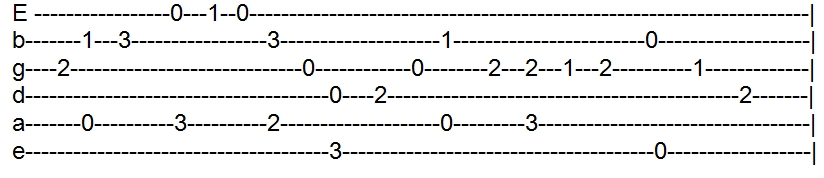
\includegraphics[width=4.75000in,height=1.03125in]{media/image31.jpeg}

b)

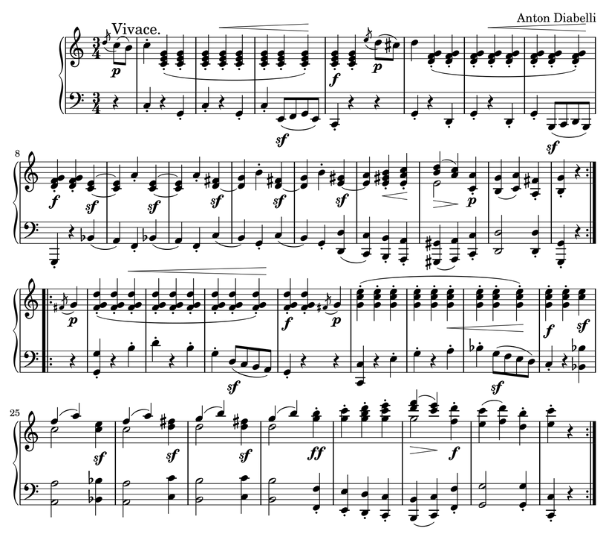
\includegraphics[width=2.76042in,height=2.43750in]{media/image32.png}

\textless{}
\url{http://pixabay.com/pt/illustrations/partitura-png-notas-musicais-1275485}\textgreater{}

c)

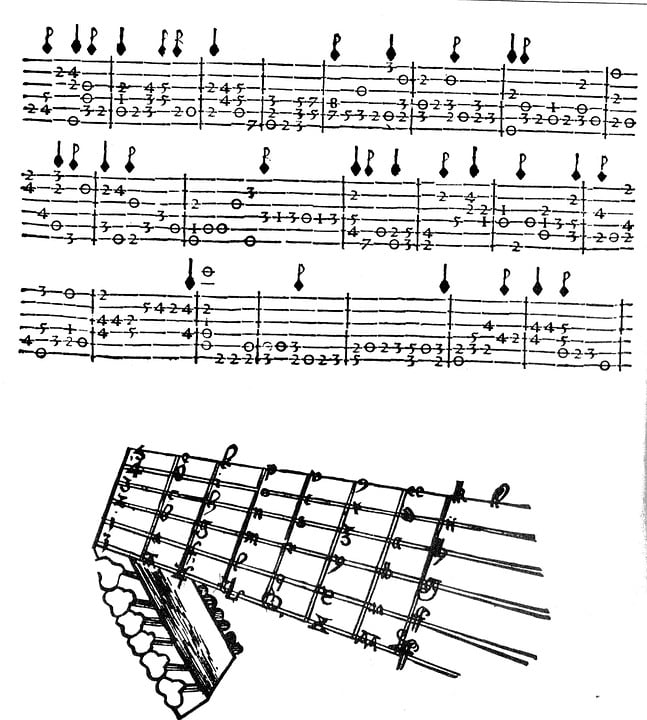
\includegraphics[width=2.59375in,height=2.88542in]{media/image33.jpeg}

\textless{}
\url{http://pixabay.com/pt/illustrations/alaúde-tablatura-música-divisória-771985}\textgreater{}

d)

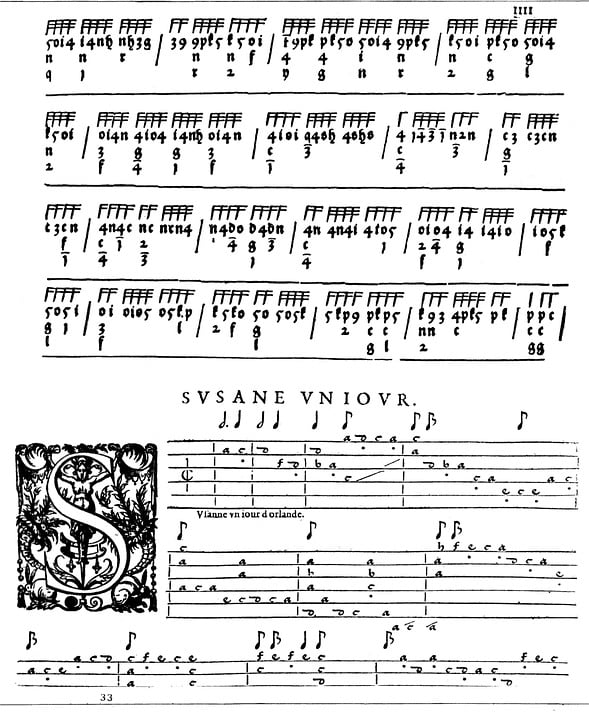
\includegraphics[width=3.13542in,height=3.83333in]{media/image34.jpeg}

\textless{}
\url{http://pixabay.com/pt/illustrations/alaúde-tablatura-música-divisória-771986}\textgreater{}

Nível: fácil.

\begin{enumerate}
\def\labelenumi{\alph{enumi})}
\item
  Incorreta. Trata-se de uma tablatura para violão, notação não
  convencional.
\item
  Correta. A notação convencional se utiliza de cinco pautas, quatro
  espaços e notas musicais.
\item
  Incorreta. Notação não convencional. Essa imagem corresponde uma
  tablatura para violão.
\item
  Incorreta. Exemplo de tablatura numérica, sistema de escrita não
  convencional, anterior ao surgimento da notação convencional que se
  utiliza de cinco pautas, quatro espaços e notas musicais.
\end{enumerate}

Saeb: - Identificar diferentes formas de registro das artes por meio de
notação ou procedimentos e técnicas de áudio e audiovisual.

BNCC: (EF69AR22) Explorar e identificar diferentes formas de registro
musical (notação musical tradicional, partituras criativas e
procedimentos da música contemporânea), bem como procedimentos e
técnicas de registro em áudio e audiovisual.

\begin{enumerate}
\def\labelenumi{\arabic{enumi}.}
\item
  Observe a imagem e leia o texto.
\end{enumerate}

\begin{longtable}[]{@{}ll@{}}
\toprule
\begin{minipage}[t]{0.48\columnwidth}\raggedright\strut
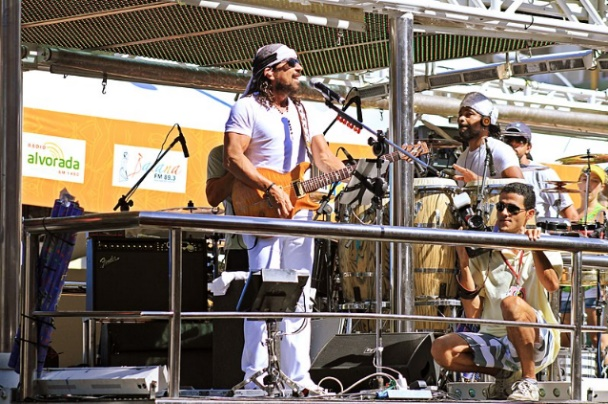
\includegraphics[width=2.76042in,height=1.83333in]{media/image35.jpeg}

\textless{}\url{https://commons.wikimedia.org/wiki/File:Bloco_Camale\%C3\%A3o_com_Chiclete_com_Banana_no_Circuito_Osmar_em_(21.02)._Foto-_Flora_Rodriguez_(6917512019).jpg}\textgreater{}\strut
\end{minipage} & \begin{minipage}[t]{0.48\columnwidth}\raggedright\strut
\emph{Chiclete com banana} é uma banda brasileira formada em 1980, que
no início de sua trajetória já tocou todo estilo de música, do rock ao
forró.\strut
\end{minipage}\tabularnewline
\bottomrule
\end{longtable}

Qual gênero musical brasileiro consagrou essa banda, principalmente, no
Carnaval de Salvador? Assinale a alternativa correta.

\begin{enumerate}
\def\labelenumi{\alph{enumi})}
\item
  Samba.
\item
  Sertanejo.
\item
  Funk.
\end{enumerate}

d) Axé.

Nível: Médio.

\begin{enumerate}
\def\labelenumi{\alph{enumi})}
\item
  Incorreta. Apesar do gênero musical samba ser um estilo de música
  muito tocado no Carnaval brasileiro, a banda Chiclete com banana se
  projetou nacionalmente com a introdução do axé em suas apresentações.
\item
  Incorreta. O sertanejo, gênero musical brasileiro, não faz parte da
  tradição do Carnaval e não é o estilo de música tocado pela banda
  \emph{Chiclete com banana}.
\item
  Incorreta. O gênero musical funk, apesar de muito tocado no Brasil,
  trata-se de um gênero com suas origens em comunidades afro-americanas
  (EUA), ou seja, não se trata de um gênero desenvolvido inicialmente no
  Brasil.
\item
  Correta. A banda Chiclete com banana iniciou sua trajetória tocando
  todo estilo de música, do rock ao forró. Mas foi com o axé que ela se
  projetou nacionalmente.
\end{enumerate}

Saeb: - Analisar o papel dos profissionais e a utilização dos
equipamentos culturais no sistema de produção e circulação das artes
visuais, dança, música e teatro.

BNCC: (EF69AR18) Reconhecer e apreciar o papel de músicos e grupos de
música brasileiros e estrangeiros que contribuíram para o
desenvolvimento de formas e gêneros musicais.

\textbf{Simulado 3}

\begin{enumerate}
\def\labelenumi{\arabic{enumi}.}
\item
  Leia o texto.
\end{enumerate}

Constituída por vários rituais religiosos e expressões culturais, é uma
celebração profundamente enraizada no cotidiano dos moradores de
Pirenópolis e determinante dos padrões de sociabilidade local. A esta
estrutura básica, os agentes vêm incorporando outros ritos e
representações, como as encenações de mascarados e cavalhadas,
responsáveis pela grande notoriedade da festa, que se realiza nesta
cidade a cada ano, desde 1819, durante cerca de 60 dias, com clímax no
Domingo de Pentecostes, cinquenta dias após a Páscoa.

Disponível em: \url{http://portal.iphan.gov.br/pagina/detalhes/72}.
Acesso em: 15 mar. 2023. (Adaptado)

A descrição do patrimônio cultural dada pelo texto refere-se

\begin{enumerate}
\def\labelenumi{\alph{enumi})}
\item
  ao Círio de Nossa Senhora de Nazaré.
\item
  à Festa do Divino Espírito Santo
\item
  à Festa do Bumba Meu Boi.
\item
  à Festa do Senhor Bom Jesus do Bonfim.
\end{enumerate}

Dificuldade: Média.

a) Incorreta. O Círio de Nossa Senhora de Nazaré é uma celebração
religiosa em Belém, Pará, tem como ponto alto a procissão.

b) Correta. Essa é uma das descrições possíveis para a Festa do Divino
Espírito Santo em Pirenópolis, Goiás.

c) Incorreta. A Festa do Bumba Meu Boi, com predominância no norte e
nordeste do Brasil, se refere às manifestações culturais e religiosas em
torno da figura do boi.

d) Incorreta. A Festa do Senhor do Bonfim é típica da cultura e da vida
social em Salvador, Bahia, e articula duas matrizes religiosas, a
católica e a afro-brasileira.

Saeb: - Avaliar produções que inter-relacionam diferentes linguagens
artísticas.

BNCC: (EF69AR34) Analisar e valorizar o patrimônio cultural, material e
imaterial, de culturas diversas, em especial a brasileira, incluindo
suas matrizes indígenas, africanas e europeias, de diferentes épocas, e
favorecendo a construção de vocabulário e repertório relativos às
diferentes linguagens artísticas.

\begin{enumerate}
\def\labelenumi{\arabic{enumi}.}
\item
  Leia o texto.
\end{enumerate}

``O Nicolas sempre teve interesse por dança. Desde muito pequenininho,
ficava dançando em casa, fazendo posturas de ioga e de contorcionismo!
Preocupados com a segurança na execução dos movimentos, meu marido e eu,
decidimos, quando ele completou 4 anos, levá-lo para uma escola de
dança, onde ele pudesse ser orientado e supervisionado por
profissionais. {[}...{]}

Fora da escola de dança, ouvimos comentários maldosos até de familiares
por ele fazer balé. Pais de colegas de escola do Nicolas também chegaram
a dizer a ele que isso não era atividade de menino e que ele se daria
melhor no futebol, lutas, hipismo... Mas nunca balé! As crianças
acabaram reproduzindo o mesmo comportamento dos pais e já fizeram
comentários como 'Mas balé é coisa de menina'.

Disponível em:
\url{https://revistacrescer.globo.com/Educacao-Comportamento/noticia/2021/04/meninos-tambem-dancam-maes-de-bailarinos-falam-sobre-preconceito.html}.
Acesso: 15 mar. 2023.

Nesse trecho de reportagem da revista \emph{Crescer}, encontra-se
destacado o depoimento de uma mãe de menino que faz aulas de balé.
Assinale a alternativa que define o tipo de estereótipo presente nos
comentários maldosos apontados pelo texto.

\begin{enumerate}
\def\labelenumi{\alph{enumi})}
\item
  Estereótipo de gênero.
\item
  Estereótipo da beleza.
\item
  Estereótipo social e econômico.
\item
  Estereótipo cultural.
\end{enumerate}

Nível: difícil.

\begin{enumerate}
\def\labelenumi{\alph{enumi}.}
\item
  Correta. Trata-se de um estereótipo de gênero, pois diz respeito à
  generalização sobre atributos e características que homens e mulheres
  possuem ou deveriam possuir.
\item
  Incorreta. O estereótipo da beleza diz respeito ao modelo padrão de
  beleza incutido na mente sobre como devem ser os aspectos físicos das
  pessoas consideradas bonitas.
\item
  Incorreta. O estereótipo social e econômico diz respeito,
  principalmente, a classe social a qual aquela pessoa pertence.
\item
  Incorreta. O estereótipo cultural está associado às culturas, etnias e
  raças.
\end{enumerate}

Saeb: - Avaliar o papel das diversas linguagens artísticas no
questionamento de estereótipos e preconceitos.

BNCC: (EF69AR33) Analisar aspectos históricos, sociais e políticos da
produção artística, problematizando as narrativas eurocêntricas e as
diversas categorizações da arte (arte, artesanato, folclore, design
etc.).

3. Leia o texto.

De acordo com a classificação da UNESCO, o Patrimônio Cultural é
composto por monumentos, grupos de edifícios ou sítios que tenham valor
universal excepcional do ponto de vista ~histórico, estético,
arqueológico, científico, etnológico ou antropológico. Incluem~obras de
arquitetura, escultura e pintura monumentais ou de caráter arqueológico,
e, ainda, obras isoladas ou conjugadas do homem e da natureza. São
denominadas~Patrimônio Natural as formações físicas, biológicas e
geológicas excepcionais,~\emph{habitats}~de espécies animais e vegetais
ameaçadas e áreas que tenham valor científico, de conservação ou
estético excepcional e universal.

Disponível em:
\url{http://portal.iphan.gov.br/pagina/detalhes/24\#:~:text=De\%20acordo\%20com\%20a\%20classifica\%C3\%A7\%C3\%A3o,\%2C\%20cient\%C3\%ADfico\%2C\%20etnol\%C3\%B3gico\%20ou\%20antropol\%C3\%B3gico}.
Acesso em: 14 mar. 2023.

Assinale a alternativa que contém um patrimônio cultural natural.

\begin{longtable}[]{@{}l@{}}
\toprule
\begin{minipage}[b]{0.97\columnwidth}\raggedright\strut
a)

Ouro Preto, Minas Gerais.

\textless{}
https://commons.wikimedia.org/wiki/File:Conjunto\_arquitet\%C3\%B4nico\_e\_urban\%C3\%ADstico\_de\_Ouro\_Preto.JPG\textgreater{}\strut
\end{minipage}\tabularnewline
\midrule
\endhead
\begin{minipage}[t]{0.97\columnwidth}\raggedright\strut
b)

Pantanal, Mato Grosso e Mato Grosso do Sul.

\textless{}
https://commons.wikimedia.org/wiki/File:Pantanal\_em\_Itiquira.jpg\textgreater{}\strut
\end{minipage}\tabularnewline
\begin{minipage}[t]{0.97\columnwidth}\raggedright\strut
c)

Paraty, Rio de Janeiro.

\textless{}
https://commons.wikimedia.org/wiki/File:Paraty\_05.JPG\textgreater{}\strut
\end{minipage}\tabularnewline
\begin{minipage}[t]{0.97\columnwidth}\raggedright\strut
d)

Cristo Redentor, Rio de Janeiro.\strut
\end{minipage}\tabularnewline
\bottomrule
\end{longtable}

Nível: fácil.

\begin{enumerate}
\def\labelenumi{\alph{enumi})}
\item
  Incorreta. Ouro Preto é um sítio urbano e a primeira cidade brasileira
  a receber o título de Patrimônio Cultural Mundial.
\item
  Correta. O Pantanal foi inscrito pela Unesco na Lista do Patrimônio
  Natural Mundial
\item
  Incorreta. Paraty é um patrimônio cultural arquitetônico e
  paisagístico.
\item
  Incorreta. O Cristo Redentor é uma estátua que faz parte da paisagem
  do Rio de Janeiro.
\end{enumerate}

Saeb: - Avaliar nas linguagens artísticas a diversidade do patrimônio
cultural da humanidade (material e imaterial), em especial o brasileiro,
a partir de suas diferentes matrizes.

BNCC: (EF69AR34) Analisar e valorizar o patrimônio cultural, material e
imaterial, de culturas diversas, em especial a brasileira, incluindo
suas matrizes indígenas, africanas e europeias, de diferentes épocas, e
favorecendo a construção de vocabulário e repertório relativos às
diferentes linguagens artísticas.

\textbf{Simulado 4}

\begin{enumerate}
\def\labelenumi{\arabic{enumi}.}
\item
  Leia o texto.
\end{enumerate}

É um local onde se encontram vestígios das pessoas que viveram no
passado. Esses vestígios revelam as atividades e a cultura de homens e
mulheres, identificados nos restos de construções, alimentação,
instrumentos de trabalho, armas, enfeites e pinturas.~

Disponível em: \url{http://portal.iphan.gov.br/pagina/detalhes/639}.
Acesso em: 16 mar. 2023.

Assinale a alternativa que corresponde à definição exposta no texto.

\begin{enumerate}
\def\labelenumi{\alph{enumi}.}
\item
  Patrimônio arqueológico.
\item
  Patrimônio paisagístico.
\item
  Patrimônio etnográfico.
\item
  Patrimônio das artes aplicadas.
\end{enumerate}

Nível: médio.

\begin{enumerate}
\def\labelenumi{\alph{enumi}.}
\item
  Correta. Fazem parte do patrimônio arqueológico os bens relacionados a
  vestígios da ocupação pré-histórica.
\item
  Incorreta. Fazem parte do patrimônio paisagístico tanto as áreas
  naturais, quanto lugares criados pelo homem aos quais é atribuído
  valor à sua configuração paisagística e que se destaquem por sua
  relação com o território onde se encontram.
\item
  Incorreta. Fazem parte do patrimônio etnográfico bens de valor
  etnográfico e de referência para grupos sociais.
\item
  Incorreta. Fazem parte do patrimônio das artes aplicadas os bens que
  têm seu valor artístico associado à função utilitária, muito comum na
  arquitetura, design e artes gráficas.
\end{enumerate}

Saeb: - Avaliar nas linguagens artísticas a diversidade do patrimônio
cultural da humanidade (material e imaterial), em especial o brasileiro,
a partir de suas diferentes matrizes.

BNCC: (EF69AR34) Analisar e valorizar o patrimônio cultural, material e
imaterial, de culturas diversas, em especial a brasileira, incluindo
suas matrizes indígenas, africanas e europeias, de diferentes épocas, e
favorecendo a construção de vocabulário e repertório relativos às
diferentes linguagens artísticas.

\begin{enumerate}
\def\labelenumi{\arabic{enumi}.}
\item
  Observe a pintura.
\end{enumerate}

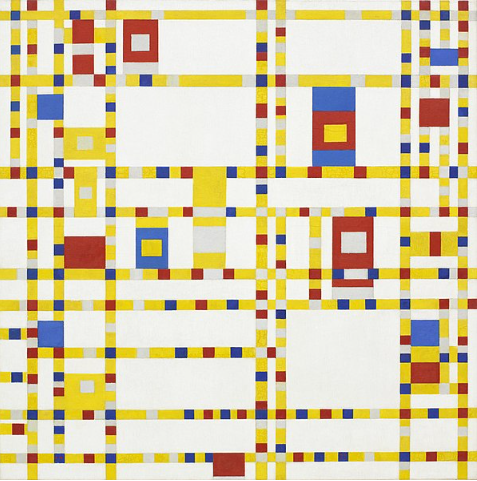
\includegraphics[width=4.96875in,height=5.01042in]{media/image40.png}

\emph{Broadway Boogie-Woogie}, 1942, de Piet Mondrian. Óleo sobre tela,
127 cm x 127 cm. Museu de Arte Moderna, Nova York, Estados Unidos da
América.

\textless{}
\url{https://commons.wikimedia.org/wiki/File:Piet_Mondrian,_1942_-_Broadway_Boogie_Woogie.jpg}\textgreater{}

A obra, de Piet Mondrian, um dos principais representantes do
abstracionismo na arte, é uma homenagem ao estilo musical
\emph{boogie-woogie}. Assinale a alternativa que contém características
dos elementos constitutivos dessa arte visual.

\begin{enumerate}
\def\labelenumi{\alph{enumi})}
\item
  Valorização de formas, cores, linhas e rejeição à perspectiva de luz e
  sombra.
\item
  Valorização da perspectiva, com técnicas de luz e sombra para dar
  profundidade e volume.
\item
  Valorização da iluminação natural, com fortes contrastes entre cor e
  luz, figuras sem contornos nítidos.
\item
  Valorização da expressão, com contornos deformados e uso de cores
  fortes e contrastantes.
\end{enumerate}

Nível: difícil.

\begin{enumerate}
\def\labelenumi{\alph{enumi})}
\item
  Correta. Segundo a descrição do texto, a artista não utilizou o gesto.
\item
  Incorreta. A perspectiva é um recurso gráfico que se utiliza de linhas
  convergentes para criar a ilusão de tridimensionalidade.
\item
  Incorreta. A luz e a sombra permitem ver as formas em volume e, sem
  esses elementos, a figura fica plana. ~
\item
  Incorreta. Os contornos não têm como característica a deformação dos
  traços.
\end{enumerate}

Saeb: - Reconhecer artistas que contribuíram para o desenvolvimento e a
disseminação de diferentes gêneros e estilos nas artes visuais, dança,
música e teatro.

BNCC: (EF69AR04) Analisar os elementos constitutivos das artes visuais
(ponto, linha, forma, direção, cor, tom, escala, dimensão, espaço,
movimento etc.) na apreciação de diferentes produções artísticas.

\begin{enumerate}
\def\labelenumi{\arabic{enumi}.}
\item
  Leia o texto.
\end{enumerate}

A fusão entre arte e tecnologia permite novos e interessantes formatos
para a criação e divulgação artísticas. O desenvolvimento tecnológico,
em especial os computadores, permitiu o surgimento de criações
artísticas que antes não eram possíveis.

Instalações artísticas, que unem imagens e sons, é apenas um exemplo de
como a arte pôde libertar-se dos suportes tradicionais (quadros e
esculturas) e agora manifestasse de maneiras inovadoras e
surpreendentes.

Ao apropriar-se das novas ferramentas tecnológicas a arte também
conseguiu sair dos museus para ganhar as ruas. Aparelhos, cada vez
menores e mais baratos, permitem que o artista exponha suas criações em
locais abertos e inusitados. Uma fachada de um prédio pode se
transformar em uma tela multimídia para a criatividade.

Disponível em: \url{https://artout.com.br/arte-e-tecnologia}. Acesso em:
16 mar. 2023.

Assinale a alternativa que contém uma característica específica das
instalações sonoras.

\begin{enumerate}
\def\labelenumi{\alph{enumi})}
\item
  Obras tridimensionais inseridas em espaços específicos.
\item
  Obras que podem explorar recursos digitais.
\item
  Obras que podem ser instaladas fora das galerias e museus.
\item
  Obras que exploram silêncio, ruído, música.
\end{enumerate}

Nível: fácil.

\begin{enumerate}
\def\labelenumi{\alph{enumi})}
\item
  Incorreta. É uma característica de instalações artísticas, mas para
  que ela seja considerada instalação sonora faz-se necessário que ela
  explore fontes e materiais sonoros na sua composição.
\item
  Incorreta. Nem todos os recursos digitais utilizados em instalações
  exploram a materialidade sonora.
\item
  Incorreta. As instalações podem ocupar ruas, praças, entre outras
  possibilidades, mas para que essa instalação em espaços
  ``alternativos'' seja considerada sonora precisa lançar mão de fontes
  e materiais sonoros.
\item
  Correta. As instalações sonoras, como o próprio nome diz, têm como
  característica determinante a exploração de fontes e materiais sonoros
  na sua criação e composição.
\end{enumerate}

Saeb: - Identificar os usos de diferentes tecnologias e recursos
digitais na produção e circulação das linguagens artísticas.

BNCC: (EF69AR21) Explorar e analisar fontes e materiais sonoros em
práticas de composição/criação, execução e apreciação musical,
reconhecendo timbres e características de instrumentos musicais
diversos.
